\documentclass[12pt, a4paper]{article}

% --- Idioma, Fontes e Codificação ---
\usepackage[utf8]{inputenc}
\usepackage[T1]{fontenc}
\usepackage[brazilian]{babel}
% \usepackage{helvet}
\usepackage{csquotes}
\usepackage{booktabs}

% --- Matemática e Física ---
\usepackage{amsmath}
\usepackage{amsfonts}
\usepackage{amssymb}
\usepackage{amsthm}
\usepackage{physics}
\usepackage{siunitx}

\AtBeginDocument{\RenewCommandCopy\qty\SI}
\ExplSyntaxOn
\msg_redirect_name:nnn { siunitx } { physics-pkg } { none }
\ExplSyntaxOff

% --- Elementos Gráficos e Layout ---
\usepackage{graphicx}
\usepackage{tikz}
\usepackage{float}
\usepackage{caption}
\usepackage{subcaption} 
\usepackage[top=2.5cm, bottom=2.5cm, left=3cm, right=3cm]{geometry}
\usepackage{enumitem}
\usepackage{adjustbox}
\usepackage{array}

% --- Sumário, Índices e Organização ---
\usepackage{verbatim}
\usepackage{makeidx}
\usepackage{sectsty}
\usepackage{tocbibind}

% --- Bibliografia (Configuração Correta) ---
\usepackage[backend=biber,style=numeric]{biblatex}
\addbibresource{refs.bib}

% --- Teoremas e Definições ---
\newtheorem{theorem}{Teorema}
\newtheorem{definition}{Definição}
\newtheorem{proposition}{Proposição}
\newtheorem{corollary}{Corolário}
\newtheorem*{remark}{Nota}

% --- Customizações de Texto ---
\newcommand{\ident}{\hspace{2em}}
\renewcommand{\figurename}{Figura}
\renewcommand{\refname}{Referências}
\renewcommand{\proofname}{\normalfont\textbf{Demonstração:}}
% \renewcommand{\thedefinition}{\Roman{definition}} 
\renewcommand{\contentsname}{Sumário}

\setlength{\parindent}{0pt}
\setlength{\parskip}{0.6em}
\setlist[itemize]{leftmargin=2.5em, labelsep=0.5em}
\setlist[enumerate]{leftmargin=2.5em, labelsep=0.5em}

% --- Links e Sumário Customizado ---
\usepackage{hyperref}
\hypersetup{
    colorlinks = true,
    linkcolor = black,
    urlcolor = cyan,
    citecolor = black
}

\makeatletter
\renewcommand\tableofcontents{
  \null\hfill\textbf{\Large\contentsname}\hfill\null\par
  \@mkboth{\MakeUppercase\contentsname}{\MakeUppercase\contentsname}
  \@starttoc{toc}
}
\makeatother


\title{Monografia}
\author{-}

\begin{document}

\maketitle
\section{Fundamentação Teórica}

% -------------------------------------------------------------------
\subsection{Da Estrutura Estática à Dinâmica: Cristalografia e Modelo de Grão Grosso}
\label{sec:grao_grosso}
% -------------------------------------------------------------------

A proteína de ligação à maltose é uma proteína bacteriana encontrada em \textit{Escherichia coli}, onde sua função primária é ligar e transportar moléculas de açúcar através das membranas celulares, fornecendo energia à bactéria \cite{Boos1998}. Embora às vezes cause doenças graves, a maioria das cepas de \textit{E.\ coli} é não patogênica e, na verdade, benéfica. Essas bactérias colonizam o trato gastrointestinal de humanos e animais e protegem o intestino de bactérias nocivas \cite{Hudault2001}. Além disso, \textit{E.\ coli} é o organismo vivo mais bem conhecido e é usado para estudar vários processos celulares \cite{VanHoudt2005}. Em nosso artigo, usamos métodos topológicos para estudar a MBP.

Enquanto realiza funções biológicas, a MBP muda sua estrutura. As 14 estruturas cristalográficas da MBP utilizadas como modelo gabarito foram obtidas por cristalografia de raios X e depositadas no \textit{Protein Data Bank} (PDB). A cristalografia de raios X é uma técnica experimental onde a proteína purificada é forçada a precipitar de uma solução até formar um cristal sólido e ordenado \cite{spurlino1991}. Quando um feixe de raios X é disparado contra esse cristal, os elétrons dos átomos da proteína difratam (espalham) os raios em várias direções. Computadores analisam o padrão e a intensidade desses feixes difratados para reconstruir um "mapa de densidade eletrônica", o que permite aos pesquisadores deduzir as coordenadas espaciais $(x,y,z)$ exatas de quase todos os átomos da biomolécula no espaço tridimensional. É essencialmente uma fotografia de alta resolução, mas estática, da proteína.

Cada estrutura da MBP contém aproximadamente 3000 átomos pesados. Trabalhar diretamente com todos eles implicaria operar num espaço de configurações $\mathbb{R}^{3 \times 3000} \cong \mathbb{R}^{9000}$, tornando inviável tanto a construção computacional do Complexo de Vietoris-Rips quanto a interpretação biológica dos invariantes topológicos obtidos \cite{cang2015topological}. A solução adotada é o \textbf{modelo de grão grosso} (\textit{coarse-grained model}): agrupam-se todos os átomos de cada resíduo de aminoácido num único nó representativo, reduzindo os 3000 átomos a $N = 370$ pontos~\cite{kovacev2016}.

\begin{definition}[Espaço de Configurações Reduzido]
Seja $N = 370$ o número de resíduos da MBP. Denota-se por $\mathbf{r}_i \in \mathbb{R}^3$ a posição do nó representativo do $i$-ésimo resíduo. Uma \emph{conformação} da proteína é o vetor de estado espacial:
$$
\mathbf{R} = (\mathbf{r}_1,\, \mathbf{r}_2,\, \ldots,\, \mathbf{r}_N) \;\in\; \mathbb{R}^{3 \times N} \;\cong\; \mathbb{R}^{1110}.
$$
O espaço de conformações termicamente acessíveis é um subespaço de $\mathbb{R}^{1110}$, e é este subespaço reduzido que a homologia persistente irá caracterizar topologicamente.
\end{definition}

O nó representativo escolhido é o \textbf{carbono-alfa} ($C_\alpha$), o átomo central do esqueleto peptídico do qual partem tanto as ligações peptídicas (que unem resíduos consecutivos) quanto as cadeias laterais (que variam entre os 20 aminoácidos). A escolha geométrica é justificada por três razões complementares atestadas na literatura estrutural:

\begin{enumerate}
    \item \textbf{Estabilidade geométrica:} as cadeias laterais apresentam grande mobilidade rotacional (ruído conformacional térmico), enquanto a cadeia principal de $C_\alpha$ forma uma curva contínua e geometricamente estável que define a topologia de contactos essenciais da proteína~\cite{cang2015}.
    \item \textbf{Redução de complexidade algorítmica:} ao focar nos $C_\alpha$, o espaço de trabalho métrico cai de $\mathbb{R}^{9000}$ para $\mathbb{R}^{1110}$, reduzindo drasticamente o custo computacional da matriz de distâncias e da subsequente filtração topológica~\cite{cang2015}.
    \item \textbf{Base para a Dinâmica de Redes:} como demonstrado formalmente por Atilgan et al.~\cite{atilgan2001}, os átomos $C_\alpha$ funcionam como os \emph{nós} da rede elástica, e as distâncias de equilíbrio entre eles representam os parâmetros geométricos estritamente necessários para construir a Matriz Hessiana do sistema mecânico.
\end{enumerate}

% -------------------------------------------------------------------
\subsection{Termodinâmica do Fechamento Conformacional e Seleção Conformacional}
\label{sec:termodinamica_fechamento}
% -------------------------------------------------------------------

A função biológica da MBP --- capturar e transportar moléculas de maltose no espaço periplasmático --- é governada por uma arquitectura estrutural altamente flexível. A proteína é composta por dois domínios globulares principais (N-terminal e C-terminal) conectados por uma região de laços flexíveis que actua como uma dobradiça (\textit{hinge}). O mecanismo de captura do ligante assemelha-se ao fechamento de uma armadilha (\textit{Venus flytrap mechanism}), resultando em alterações geométricas macroscópicas na estrutura da macromolécula~\cite{spurlino1991}.

Estudos baseados em cristalografia de raios X e dinâmica molecular, como os conduzidos por Bucher et al.~\cite{bucher2011}, classificam as conformações da MBP em três macrostados estruturais principais (ver Figura~\ref{fig:mbp_conformations}):

\begin{enumerate}
    \item \textbf{Estado Aberto (\textit{Open}):} Caracteriza-se por uma grande separação angular e espacial entre os dois domínios globulares. É a forma predominante da proteína no estado \textit{apo} (livre de ligante), representando o mínimo global de energia do sistema na ausência do açúcar.
    \item \textbf{Estado Semi-fechado (\textit{Semi-closed}):} Um estado intermediário transiente. A estrutura apresenta um fechamento parcial da fenda interdominial.
    \item \textbf{Estado Fechado (\textit{Closed}):} Os domínios globulares aproximam-se significativamente, engolfando completamente o ligante na fenda catalítica. Este é o estado funcional ativo, frequentemente associado à forma \textit{holo} (ligada à maltose).
\end{enumerate}

\begin{figure}[H]
    \centering
    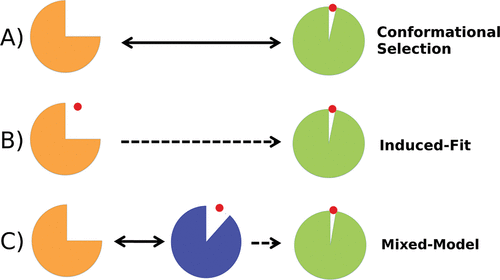
\includegraphics[width=0.8\textwidth]{conformidade_proteina.png} 
    \caption{Representação das transições conformacionais da MBP. Da esquerda para a direita: Estado Aberto, Semi-fechado transiente e Fechado estabilizado pelo ligante (em vermelho). Fonte: Adaptado de Bucher et al.~\cite{bucher2011}.}
    \label{fig:mbp_conformations}
\end{figure}

Historicamente, assumia-se que a transição do estado aberto para o fechado era estritamente induzida pelo impacto mecânico da entrada da maltose na fenda (modelo de \textit{Encaixe Induzido}). Contudo, a biofísica estrutural contemporânea demonstra que a MBP opera sob o princípio da \textbf{Seleção Conformacional}~\cite{Seeliger2010}. Segundo este modelo, a proteína não é estática; ela "respira" e oscila naturalmente entre as formas aberta e semi-fechada através de flutuações térmicas, mesmo sem a presença do ligante. 

O papel da maltose, portanto, não é forçar o fechamento da dobradiça, mas sim \emph{estabilizar} a forma fechada pré-existente. Quando o ligante se aloja na fenda, ele estabelece uma rede complexa de ligações de hidrogénio que compensa a tensão elástica da proteína, tornando a conformação fechada termodinamicamente favorável~\cite{bucher2011}. 

É precisamente esta vasta gama de flutuações e movimentos cooperativos de dobradiça --- que ocorrem independentemente da presença do açúcar --- que torna a geometria euclidiana estática insuficiente para classificar as proteínas. Para mapear com rigor estes padrões de oscilação em trajectórias matemáticas, o sistema deve ser modelado através das suas interações de rede elástica.

Em \cite{kovacev2016} é coletado um conjunto de 14 proteínas, separadas em: sete conformações fechadas e sete conformações abertas. Há uma diferença entre elas usando energias de deformação; a conformação fechada energeticamente mais favorável liga uma molécula de açúcar, enquanto sua contraparte aberta requer maiores energias de deformação e pode ou não se envolver no processo de ligação. A lista das quatorze estruturas da MBP que foram investigadas é mostrada na Tabela~\ref{tab:estruturas}.

\begin{table}[H]
    \centering
    \captionsetup{margin=1cm}

    \begin{adjustbox}{max width=\textwidth}
        % Corrigido de cccllc (6 colunas) para ccllc (5 colunas)
        \begin{tabular}{@{}ccllc@{}}
            \toprule
            \textbf{Nº} & \textbf{Código PDB} & \textbf{Nome do Ligante} & \textbf{Estrutura da Proteína} & \textbf{Referência} \\
            \midrule
            1  & 1ANF & maltose        & fechada-\textit{holo} & Quiocho et al.\ (1997) \\
            2  & 1FQC & maltotriotol   & fechada-\textit{holo} & Duan et al.\ (2001)   \\
            3  & 1FQD & maltotetraitol & fechada-\textit{holo} & Duan et al.\ (2001)   \\
            4  & 1MPD & maltose        & fechada-\textit{holo} & Shilton et al.\ (1996) \\
            5  & 3HPI & sacarose       & fechada-\textit{holo} & Gould \& Shilton (2010) \\
            6  & 3MBP & maltotriose    & fechada-\textit{holo} & Quiocho et al.\ (1997) \\
            7  & 4MBP & maltotetraose  & fechada-\textit{holo} & Quiocho et al.\ (1997) \\
            8  & 1EZ9 & maltetetraitol & aberta-\textit{holo}  & Duan \& Quiocho (2002) \\
            9  & 1FQA & maltotetraitol & aberta-\textit{holo}  & Duan et al.\ (2001)   \\
            10 & 1FQB & maltotetraitol & aberta-\textit{holo}  & Duan et al.\ (2001)   \\
            11 & 1JW4 & ---            & aberta-\textit{apo}   & Duan \& Quiocho (2002) \\
            12 & 1JW5 & maltose        & aberta-\textit{holo}  & Duan \& Quiocho (2002) \\
            13 & 1LLS & ---            & aberta-\textit{apo}   & Rubin et al.\ (2002)  \\
            14 & 1OMP & ---            & aberta-\textit{apo}   & Sharff et al.\ (1992) \\
            \bottomrule
        \end{tabular}
    \end{adjustbox}
    \caption{Tabela retirada de \cite{kovacev2016}. Quatorze estruturas da MBP com os nomes dos ligantes para as formas \textit{holo}. Cada estrutura é identificada por um código de quatro letras do Protein Data Bank \cite{Bernstein1977}.}
    \label{tab:estruturas}
\end{table}


% -------------------------------------------------------------------
\subsection{O Formalismo da Rede Anisotrópica (ANM) e a Matriz Hessiana Estrutural}
\label{sec:anm}
% -------------------------------------------------------------------

Para mapear com rigor analítico as flutuações e os movimentos cooperativos de dobradiça da MBP, faz-se necessário transcender as descrições estáticas e adotar um modelo mecânico das interações moleculares. O fundamento teórico para modelar as flutuações direcionais tridimensionais repousa sobre o formalismo do Modelo de Rede Anisotrópica (\textit{Anisotropic Network Model} -- ANM), introduzido pelo estudo seminal de Atilgan et al.~\cite{atilgan2001}. Este modelo supera as limitações topológicas clássicas do Modelo de Rede Gaussiana (\textit{Gaussian Network Model} -- GNM) o qual, por ser puramente escalar, pressupõe flutuações isotrópicas e omite as preferências direcionais dos resíduos ao longo dos eixos cartesianos.

\subsubsection{Formulação Tridimensional da Energia Potencial Elástica}

No âmbito do ANM, a arquitectura estrutural da MBP ($N = 370$ resíduos) é convertida num sistema mecânico de grão grosso. Pares de nós (carbonos-alfa) cujas distâncias geométricas na estrutura cristalográfica de equilíbrio sejam inferiores a um raio de corte termodinâmico ($r_c$, tipicamente parametrizado entre $13$ e $15$~\AA) são modelados como se estivessem conectados por molas harmónicas virtuais submetidas a uma constante de força fenomenológica uniforme $\gamma$.

Sejam $\mathbf{r}_i = (X_i, Y_i, Z_i)^T$ e $\mathbf{r}_j = (X_j, Y_j, Z_j)^T$ os vetores posição instantâneos dos resíduos $i$ e $j$ sob agitação térmica, e $\mathbf{r}_i^0, \mathbf{r}_j^0$ as suas respectivas coordenadas de relaxamento (equilíbrio) obtidas via cristalografia. A distância instantânea é definida pela norma euclidiana $s_{ij} = |\mathbf{r}_{ij}| = |\mathbf{r}_j - \mathbf{r}_i|$, enquanto a distância de relaxamento elástico é dada por $s_{ij}^0 = |\mathbf{r}_{ij}^0| = |\mathbf{r}_j^0 - \mathbf{r}_i^0|$. 

Sob a aproximação harmónica para pequenas flutuações, a energia potencial total de deformação do sistema mecânico, $V_{\text{total}}$, é expressa pelo somatório escalar das contribuições elásticas par a par:

\begin{equation}\label{eq:potencial_anm_completo}
    V_{\text{total}} = \frac{\gamma}{2} \sum_{i=1}^{N-1} \sum_{j=i+1}^{N} \left[ \sqrt{(X_j - X_i)^2 + (Y_j - Y_i)^2 + (Z_j - Z_i)^2} - s_{ij}^0 \right]^2 \mathbf{1}_{[(i,j) \in \mathcal{E}]},
\end{equation}

onde $\mathcal{E}$ define o conjunto de contactos topológicos intrínsecos determinado pelo raio de corte, de modo que a função indicadora $\mathbf{1}_{[(i,j) \in \mathcal{E}]} = 1$ se, e somente se, $s_{ij}^0 \leq r_c$, assumindo o valor $0$ caso contrário.

\subsubsection{Construção Analítica da Matriz Hessiana}

O comportamento dinâmico e as forças de restituição do sistema linearizado em torno do mínimo global de energia elástica são inteiramente mapeados pela matriz Hessiana estrutural, denotada por $\mathbf{H} \in \mathbb{R}^{3N \times 3N}$. A matriz $\mathbf{H}$ é construída através da expansão em série de Taylor de segunda ordem do potencial $V_{\text{total}}$ e é estruturada matematicamente em $N \times N$ sub-blocos (ou super-elementos) de dimensão $3 \times 3$.

Cada sub-bloco $\mathbf{H}_{ij}$ encapsula as segundas derivadas parciais do potencial elástico em relação às componentes cartesianas dos deslocamentos espaciais dos nós $i$ e $j$. Para os super-elementos \emph{fora da diagonal principal} ($i \neq j$), que calculam o acoplamento mecânico direcional da mola entre dois resíduos distintos, a diferenciação analítica da Equação~\eqref{eq:potencial_anm_completo} avaliada na configuração de equilíbrio resulta na seguinte matriz Jacobiana de interações:

\begin{equation}\label{eq:hessiana_off_diagonal}
\begin{aligned}
    \mathbf{H}_{ij} &= \begin{bmatrix}
    \frac{\partial^2 V}{\partial X_i \partial X_j} & \frac{\partial^2 V}{\partial X_i \partial Y_j} & \frac{\partial^2 V}{\partial X_i \partial Z_j} \\[6pt]
    \frac{\partial^2 V}{\partial Y_i \partial X_j} & \frac{\partial^2 V}{\partial Y_i \partial Y_j} & \frac{\partial^2 V}{\partial Y_i \partial Z_j} \\[6pt]
    \frac{\partial^2 V}{\partial Z_i \partial X_j} & \frac{\partial^2 V}{\partial Z_i \partial Y_j} & \frac{\partial^2 V}{\partial Z_i \partial Z_j}
    \end{bmatrix}
\end{aligned}
\end{equation}

A expressão~\eqref{eq:hessiana_off_diagonal} pode ser escrita de forma elegante através do produto externo (\textit{outer product}) do vetor de distância geométrica $\mathbf{r}_{ij}^0$:

\begin{equation}\label{eq:hessiana_off_diagonal_compacta}
\mathbf{H}_{ij} = -\frac{\gamma}{(s_{ij}^0)^2} (\mathbf{r}_{ij}^0)(\mathbf{r}_{ij}^0)^T \mathbf{1}_{[(i,j) \in \mathcal{E}]}.
\end{equation}

Inversamente, os super-elementos localizados na \emph{diagonal principal} da Hessiana ($\mathbf{H}_{ii}$) não modelam uma interação individual, mas sim a soma vetorial das forças de reação elástica exercidas por todas as molas conectadas ao $i$-ésimo nó. Por imperativo da terceira lei de Newton e da conservação do momento linear (invariância translacional), a diagonal é rigorosamente definida pelo balanço negativo das interações circundantes:

\begin{equation}\label{eq:hessiana_diagonal}
\mathbf{H}_{ii} = - \sum_{j \neq i}^N \mathbf{H}_{ij}.
\end{equation}

A matriz global $\mathbf{H}$ assim construída é simétrica e semidefinida positiva, abrigando toda a topologia de conectividade e as anisotropias mecânicas que definem o estado termodinâmico da MBP.

% -------------------------------------------------------------------
\subsection{Decomposição Espectral, Truncamento e a Correlação Cruzada}
\label{sec:decomposicao_espectral}
% -------------------------------------------------------------------

A matriz Hessiana $\mathbf{H} \in \mathbb{R}^{3N \times 3N}$, derivada na secção anterior, contém a totalidade da informação sobre o panorama de flutuações da proteína ao redor do seu estado de equilíbrio. Sendo $\mathbf{H}$ uma matriz real, simétrica e semidefinida positiva, o seu comportamento termodinâmico pode ser dissecado resolvendo o problema de autovalores, o que equivale a realizar uma transformação ortogonal de coordenadas conhecida como decomposição espectral.

\subsubsection{Modos Normais e Truncamento de Baixa Frequência}

A diagonalização da matriz Hessiana fornece um conjunto completo de $3N$ autovalores $\lambda_k$ e os seus respetivos autovetores ortonormais $\mathbf{u}_k \in \mathbb{R}^{3N}$:

\begin{equation}\label{eq:diagonalizacao}
\mathbf{H} = \sum_{k=1}^{3N} \lambda_k \mathbf{u}_k \mathbf{u}_k^T.
\end{equation}

Fisicamente, os autovalores estão diretamente relacionados com a rigidez direcional e são proporcionais ao quadrado das frequências vibracionais dos modos normais ($\lambda_k \propto \omega_k^2$). Os autovetores $\mathbf{u}_k$ descrevem a forma geométrica (direção e amplitude) do deslocamento coletivo dos resíduos sob aquele específico modo de vibração.

Devido à invariância translacional e rotacional da molécula inteira como um corpo rígido livre no espaço tridimensional, os primeiros seis autovalores ($k = 1, \ldots, 6$) são estritamente nulos ($\lambda_k = 0$). Restam, portanto, $3N - 6 = 1104$ modos físicos não-triviais de oscilação interna.

A conexão matemática entre este arcabouço biofísico e a metodologia estatística delineada por Kovacev-Nikolic et al.~\cite{kovacev2016} estabelece-se por meio do \textbf{truncamento espectral}. Autovalores de grande magnitude correspondem a movimentos rápidos, locais e de alta frequência (tais como estiramentos de ligações covalentes pontuais), que representam mero ruído termodinâmico na perspetiva da transição funcional da proteína.

Para capturar exclusivamente a mecânica cooperativa global --- isto é, o movimento de dobradiça (\textit{hinge-bending}) essencial para a captura da maltose ---, opera-se uma restrição do espaço dimensional. Filtram-se as vibrações atómicas de alta frequência e retêm-se apenas os primeiros $M = 20$ modos não-triviais de menor autovalor ($k = 7, \ldots, 26$). A matriz pseudoinversa de Moore-Penrose truncada, $\mathbf{H}^+_{\text{trunc}}$, é reconstruída estritamente sobre este subespaço funcional de baixa frequência:

\begin{equation}\label{eq:pseudoinversa_truncada}
\mathbf{H}^+_{\text{trunc}} = \sum_{k=7}^{7+M-1} \frac{1}{\lambda_k} \mathbf{u}_k \mathbf{u}_k^T.
\end{equation}

\subsubsection{Derivação da Matriz de Correlação Cruzada}

Sob a aproximação de que as flutuações conformacionais ($\Delta\mathbf{R}$) seguem uma distribuição multivariada exata de Boltzmann, Atilgan et al.~\cite{atilgan2001} demonstram que a covariância termodinâmica entre as flutuações espaciais dos resíduos $i$ e $j$ é diretamente proporcional aos sub-blocos $3 \times 3$ da matriz pseudoinversa. 

O produto interno termodinâmico (covariância cruzada) é obtido calculando o traço ($\mathrm{Tr}$), ou seja, a soma dos elementos da diagonal principal, do respetivo sub-bloco $[\mathbf{H}^+_{\text{trunc}}]_{ij}$:

\begin{equation}\label{eq:covariancia}
\langle \Delta\mathbf{r}_i \cdot \Delta\mathbf{r}_j \rangle = k_B T \, \mathrm{Tr}\left(\left[\mathbf{H}^+_{\text{trunc}}\right]_{ij}\right),
\end{equation}

onde $k_B$ é a constante de Boltzmann e $T$ a temperatura absoluta. Para isolar a pureza direcional do movimento e anular as diferenças de magnitude absoluta das flutuações, normaliza-se esta covariância. Define-se assim a \textbf{correlação cruzada dinâmica normalizada} ($C_{ij}$) entre qualquer par de resíduos na proteína:

\begin{equation}\label{eq:correlacao}
C_{ij} = \frac{\mathrm{Tr}\left(\left[\mathbf{H}^+_{\text{trunc}}\right]_{ij}\right)} {\sqrt{\mathrm{Tr}\left(\left[\mathbf{H}^+_{\text{trunc}}\right]_{ii}\right)\,\mathrm{Tr}\left(\left[\mathbf{H}^+_{\text{trunc}}\right]_{jj}\right)}}, \qquad C_{ij} \in [-1,\,1].
\end{equation}

Esta matriz de correlação $\mathbf{C} \in \mathbb{R}^{N \times N}$ destila a totalidade da coreografia mecânica da MBP: valores positivos próximos de $1$ denotam resíduos que se deslocam de forma coordenada na mesma direção; valores negativos próximos de $-1$ identificam resíduos em oposição de fase (anticorrelação, agindo como os braços opostos de uma alavanca); e valores nulos indicam independência cinemática e ausência de comunicação alostérica.

% -------------------------------------------------------------------
\subsection{Transição Métrica: Da Geometria Euclidiana à Topologia Dinâmica}
\label{sec:metrica_topologica}
% -------------------------------------------------------------------

O emprego clássico da Análise Topológica de Dados (TDA) em biologia estrutural baseia-se frequentemente nas coordenadas espaciais cartesianas $(X, Y, Z)$ para construir o espaço métrico subjacente. Contudo, como estabelecido nas secções anteriores, as coordenadas obtidas por cristalografia de raios X fornecem apenas uma estrutura média termodinâmica da molécula. Visto que a função de captura do ligante pela MBP depende intrinsecamente das flutuações ao longo do tempo, o descarte deliberado da distância euclidiana pura em favor de um descritor dinâmico é estritamente necessário~\cite{kovacev2016}.

Para preparar os dados das flutuações para a construção do complexo de Vietoris-Rips, utiliza-se a transformação linear da matriz de correlação cruzada normalizada $\mathbf{C}$ (Equação~\ref{eq:correlacao}) na matriz de distâncias dinâmicas $\mathbf{D}$ (Equação~\ref{eq:distancia_dinamica}). Esta nova matriz é definida elemento a elemento pela relação:

\begin{equation}\label{eq:distancia_dinamica}
D_{ij} = 1 - |C_{ij}|.
\end{equation}

Esta conversão mapeia o domínio de $[-1, 1]$ da correlação para um espaço pseudométrico rigoroso $[0, 1]$, carregando implicações estatísticas e topológicas profundas.

\subsubsection{O Significado Probabilístico e a Pseudométrica}

\ident Sob a óptica da teoria das probabilidades~\cite{devore2012}, o coeficiente de correlação é um estimador paramétrico que quantifica a força e a direção da dependência linear entre duas variáveis aleatórias. A aplicação do valor absoluto acoplada ao deslocamento linear em~\eqref{eq:distancia_dinamica} promove um reescalonamento probabilístico exacto:

\begin{itemize}
    \item \textbf{Alta Dependência Cinemática ($|C_{ij}| \to 1$):} A operação de módulo confere o mesmo peso analítico tanto à correlação perfeitamente positiva (movimento uníssono no mesmo sentido) quanto à anticorrelação extrema (movimento em sentidos opostos, como as alavancas de uma tesoura). Neste limite, a distância atribuída tende a zero ($D_{ij} \to 0$). Probabilisticamente, isto atesta um elevado grau de determinismo: conhecer o vetor de deslocamento termodinâmico do resíduo $i$ determina de forma perfeitamente previsível a resposta mecânica do resíduo $j$.
    \item \textbf{Independência e Ruído Térmico ($C_{ij} \to 0$):} Se as vibrações mecânicas de dois resíduos são ortogonais ou governadas por ruído térmico aleatório e independente, a relação linear anula-se. Consequentemente, a equação devolve a distância matemática máxima estipulada pelo modelo ($D_{ij} \to 1$).
\end{itemize}

A matriz $\mathbf{D}$ satisfaz as propriedades de não-negatividade ($D_{ij} \geq 0$), simetria ($D_{ij} = D_{ji}$) e identidade dos indiscerníveis ($D_{ii} = 0$). A desigualdade triangular ($D_{ik} \leq D_{ij} + D_{jk}$) é matematicamente garantida pelo facto de $|C_{ij}|$ derivar de um produto interno num espaço de Hilbert de flutuações, decorrendo assim da desigualdade de Cauchy-Schwarz. Estas propriedades validam $\mathbf{D}$ como uma pseudométrica fidedigna.

% -------------------------------------------------------------------
\subsection{Redução de Dimensionalidade e Visualização do Espaço de Comunicação: ISOMAP}
\label{sec:isomap_scree}
% -------------------------------------------------------------------

A construção da matriz de distâncias dinâmicas $\mathbf{D} \in \mathbb{R}^{N \times N}$ (onde $N=370$ resíduos) dota a proteína de uma nova geometria topológica, fundamentalmente distinta da sua estrutura física. Neste novo espaço métrico de dimensão $N$, os resíduos que se movem de forma termodinamicamente coordenada estão próximos (distância tendendo a zero), independentemente de quão distantes estejam na estrutura cristalográfica original em $\mathbb{R}^3$. 

Contudo, $\mathbf{D}$ é um objeto de alta dimensionalidade. Para que seja possível inspecionar visualmente este \enquote{espaço de comunicação} e extrair a sua estrutura global latente, é imperativo aplicar técnicas de redução de dimensionalidade. O objetivo matemático subjacente é encontrar um conjunto de coordenadas de baixa dimensão $\mathbf{Y} = \{\mathbf{y}_1, \ldots, \mathbf{y}_N\} \subset \mathbb{R}^d$ (com $d \ll N$) de modo que a distância euclidiana neste novo subespaço mapeie o mais fielmente possível a distância dinâmica original, ou seja, $\|\mathbf{y}_i - \mathbf{y}_j\|_{\mathbb{R}^d} \approx D_{ij}$.

\subsubsection{A Limitação do MDS Clássico}

A abordagem analítica padrão para este problema de imersão métrica é o \textit{Multidimensional Scaling} Clássico (MDS). O MDS opera transformando a matriz de distâncias ao quadrado $\mathbf{D}^{(2)}$ numa matriz de produtos internos (matriz de Gram) através de um operador de dupla centralização (\textit{double centering}):

\begin{equation}\label{eq:mds_centering}
\mathbf{B} = -\frac{1}{2} \mathbf{H} \mathbf{D}^{(2)} \mathbf{H}, \qquad \text{onde } \mathbf{H} = \mathbf{I} - \frac{1}{N}\mathbf{1}\mathbf{1}^T,
\end{equation}

sendo $\mathbf{I}$ a matriz identidade de ordem $N$ e $\mathbf{1}$ um vetor coluna de uns. Em seguida, realiza-se a decomposição espectral $\mathbf{B} = \mathbf{V} \mathbf{\Lambda} \mathbf{V}^T$ e retêm-se os $d$ maiores autovalores para construir as coordenadas projetadas.

No entanto, conforme reportado por Kovacev-Nikolic et al.~\cite{kovacev2016}, o MDS apresenta erros residuais elevados ao lidar com a dinâmica da MBP. A justificativa rigorosa para esta falha reside no facto de o MDS assumir que os dados residem num subespaço global \emph{linear} (um hiperplano rígido). A dinâmica conformacional de uma proteína, guiada por potenciais harmónicos locais e barreiras estéricas, desenvolve-se sobre uma \emph{variedade não-linear} (\textit{manifold}) intrincada e curva no espaço de fase. Ao tentar preservar todas as distâncias globais por meio de linhas retas euclidianas intrínsecas ao modelo linear, o MDS cria "curtos-circuitos" através de regiões do espaço que são termodinamicamente inatingíveis para a estrutura real da proteína.

\subsubsection{A Solução via ISOMAP e Distâncias Geodésicas}

Para mitigar a distorção imposta pelas projeções lineares, o estudo adota o \textbf{ISOMAP} (\textit{Isometric Mapping})~\cite{Tenenbaum2000}. O ISOMAP é uma técnica de \textit{manifold learning} que generaliza o MDS clássico, substituindo as métricas euclidianas diretas por \textbf{distâncias geodésicas} — isto é, as distâncias medidas estritamente \emph{ao longo da superfície} curvada da variedade dos dados. O rigor do algoritmo ISOMAP desdobra-se em três etapas computacionais:

\begin{enumerate}
    \item \textbf{Construção do Grafo de Vizinhança Local:} Define-se um grafo ponderado $G = (V, E)$, onde os vértices são os $N$ resíduos. Uma aresta conecta o nó $i$ ao nó $j$ apenas se estes forem vizinhos próximos sob a matriz dinâmica $\mathbf{D}$ (por norma, através do algoritmo dos $k$-vizinhos mais próximos ou de uma bola limitante de raio $\epsilon$). O peso da aresta é o próprio valor $D_{ij}$. Esta etapa captura a topologia local onde o espaço pode ser aproximado por um plano linear.
    \item \textbf{Cálculo Global das Geodésicas:} Para resíduos distantes, a separação não é ditada pela matriz original $\mathbf{D}$ (que poderia causar um curto-circuito não-linear), mas sim pela acumulação dos caminhos mais curtos através do grafo local $G$. Recorrendo a algoritmos de optimização em grafos (como Dijkstra ou Floyd-Warshall), constrói-se a matriz de distâncias geodésicas $\mathbf{D}^{(G)}$:
    \begin{equation*}\label{eq:geodesica}
    D^{(G)}_{ij} = \min_{\text{caminho } p} \left( \sum_{e \in p} \text{peso}(e) \right).
    \end{equation*}
    \item \textbf{Imersão Métrica (MDS Geodésico):} O operador do MDS Clássico (Equação~\ref{eq:mds_centering}) é, por fim, aplicado estritamente sobre a matriz geodésica não-linear $\mathbf{D}^{(G)}$, gerando o espectro de coordenadas de baixa dimensão $\mathbf{Y}$ que desdobra (\textit{unfolds}) e preserva a topologia curva intrínseca.
\end{enumerate}

O ISOMAP exibe erros residuais substancialmente menores que o MDS porque respeita a continuidade dos movimentos biológicos: a correlação alostérica entre domínios distantes da MBP é forçada a fluir através da malha de aminoácidos intermédios conectados.

\subsubsection{Dimensionalidade Intrínseca e o Gráfico Scree (Cotovelo)}

A determinação empírica da dimensão alvo $d$ para a projeção final $\mathbf{Y} \in \mathbb{R}^d$ exige a avaliação da \textbf{dimensionalidade intrínseca} da variedade subjacente — o número mínimo de eixos latentes indispensáveis para encapsular a totalidade da informação estrutural sem introduzir ruído ou aglomeração espúria (\textit{crowding problem}).

Para avaliar a fidelidade da redução, quantifica-se o \textit{stress} topológico, formulado pela variância residual do mapeamento. Trata-se de uma função estritamente decrescente da dimensão $d$, dada por:

\begin{equation*}\label{eq:variancia_residual}
\text{Variância Residual}(d) = 1 - R^2\left(\text{vec}(\mathbf{D}^{(G)}), \, \text{vec}(\mathbf{D}_{\mathbf{Y}}^{(d)})\right),
\end{equation*}

onde $R^2$ representa o coeficiente de correlação linear (o quadrado da correlação de Pearson) calculado entre o vetor de distâncias geodésicas originais e as distâncias euclidianas estimadas no subespaço de dimensão $d$ ($\mathbf{D}_{\mathbf{Y}}^{(d)}$).

A análise do comportamento assintótico desta métrica em função do número sucessivo de dimensões $d$ projeta-se visualmente no designado \textbf{Gráfico Scree} (\textit{Scree Plot}). A extração da dimensão ótima assenta no \textbf{Critério do Cotovelo} (\textit{Elbow Method}). Este critério geométrico identifica o hiperparâmetro de transição (o "cotovelo" da curva) onde a taxa de mitigação do erro residual sofre uma flexão abrupta e passa a assemelhar-se a um platô assintótico horizontal.

Conforme evidenciado pelas matrizes dinâmicas da MBP estudadas por Kovacev-Nikolic et al.~\cite{kovacev2016} (Figura 3 do respetivo artigo), o declínio acentuado das distorções de mapeamento termina precisamente quando $d = 3$. A incorporação de autovetores sucessivos para gerar uma quarta ou quinta dimensão induz ganhos marginais e irrisórios no coeficiente de determinação $R^2$. Esta observação matemática corrobora a tese de que a imensa complexidade dinâmica estabelecida pelos 370 resíduos macromoleculares pode ser otimizadamente embutida num subespaço denso de três dimensões ($\mathbb{R}^3$). É neste prisma reduzido e fiel à mecânica da proteína que as nuvens de pontos de interações se revelam preparadas para a subsequente análise de agrupamentos de classes (\textit{apo} versus \textit{holo}).

\begin{figure}[H]
    \centering
    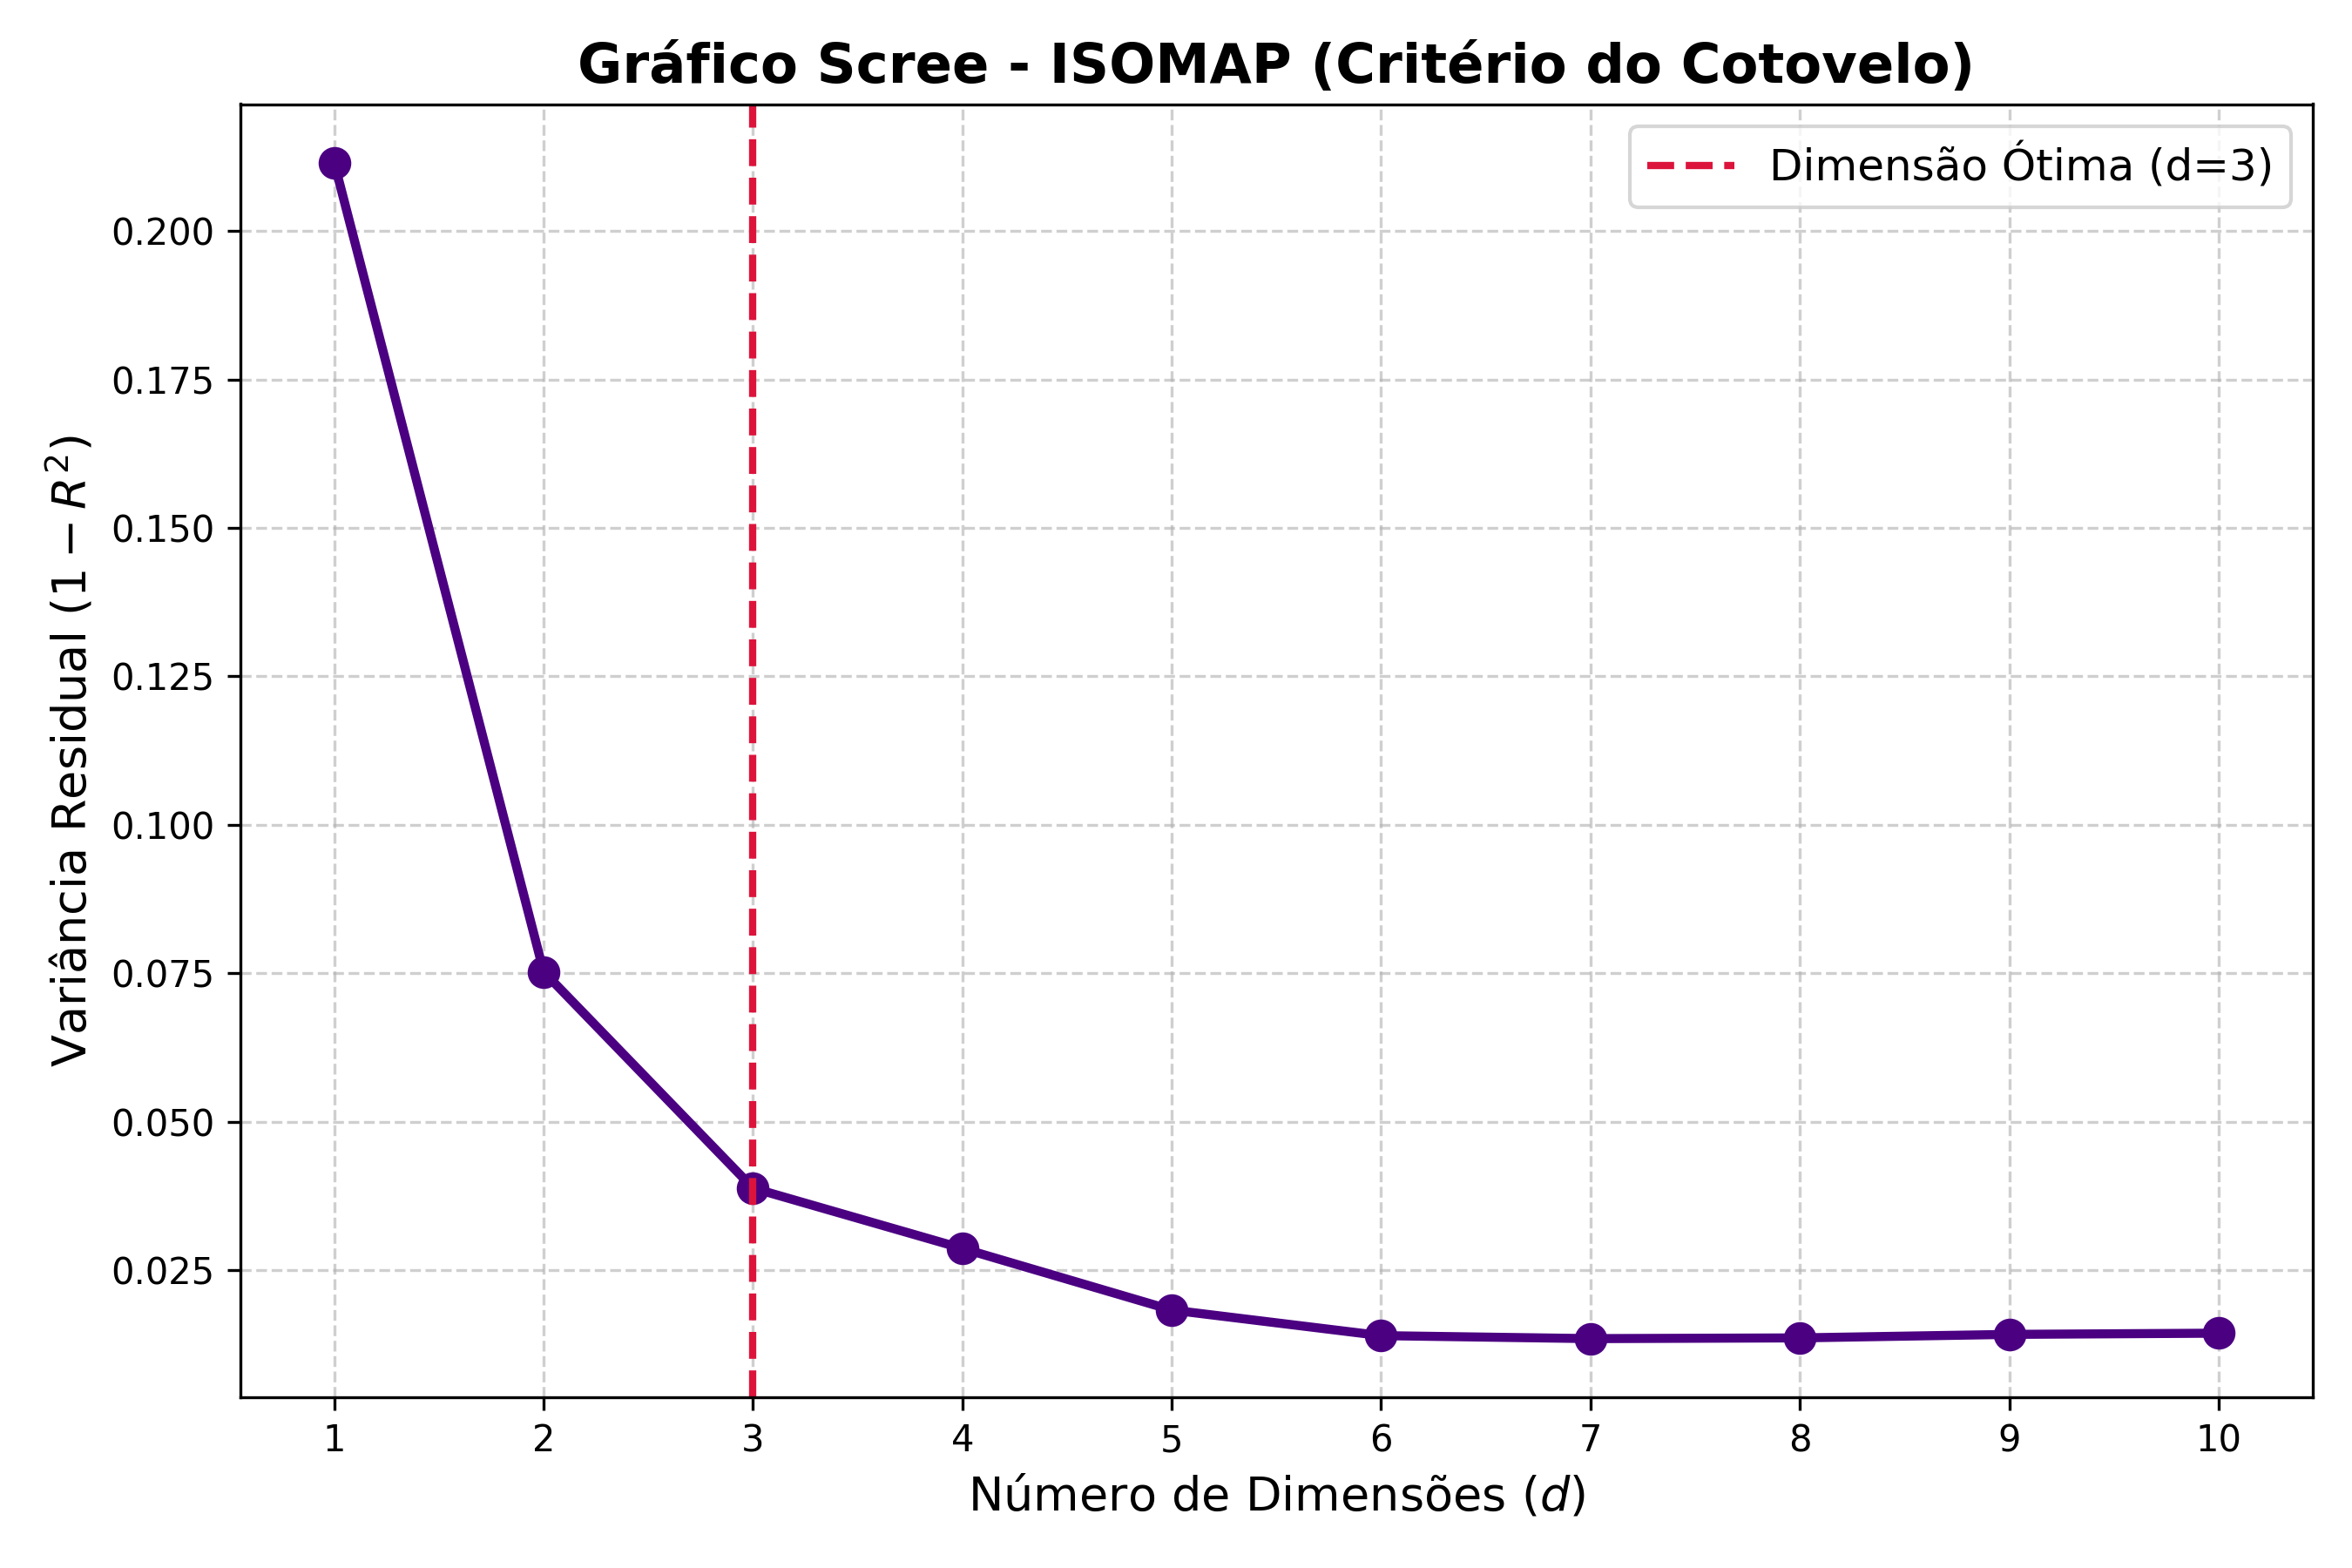
\includegraphics[width=0.8\textwidth]{grafico_scree_isomap.png}
    
    \caption{ Redução de dimensão via Isomap para a estrutura 1OMP. A flexão abrupta no parâmetro $d=3$ (Critério do Cotovelo) indica a dimensionalidade intrínseca ideal para a representação das flutuações dinâmicas da MBP.}
    \label{fig:grafico_scree} 
\end{figure}

% -------------------------------------------------------------------
\subsection{Definições Topológicas e a Geometria da Comunicação Dinâmica}
\label{sec:topologia_dinamica}
% -------------------------------------------------------------------

O emprego clássico da Análise Topológica de Dados (TDA) em biologia estrutural baseia-se frequentemente nas coordenadas espaciais cartesianas $(X, Y, Z)$ para construir o espaço métrico subjacente. Contudo, visto que a função de captura do ligante pela MBP depende intrinsecamente das flutuações térmicas ao longo do tempo, a distância euclidiana pura fornece apenas um instantâneo estático. Torna-se, portanto, estritamente necessário substituir essa geometria por um descritor dinâmico~\cite{kovacev2016}.

\subsubsection{Fundamentos de Topologia Algébrica}

Para extrair a arquitectura de comunicação da biomolécula a partir desta pseudométrica, traduzimos este espaço num objecto combinatório. Seja $K$ um complexo simplicial abstracto. Para $n \geq 0$, definimos os conjuntos
\begin{align*}
    K_n &= \{\sigma \in K \mid \dim(\sigma) \leq n\}\\
    K_{(n)} &= \{\sigma \in K \mid \dim(\sigma) = n\}. 
\end{align*}
O primeiro conjunto é um complexo simplicial, chamado de $n$-esqueleto de $K$. O segundo não é um complexo simplicial em geral.

\begin{definition}[Complexo Simplicial]
Seja $V$ um conjunto (chamado de conjunto de vértices). Um \textbf{complexo simplicial} sobre $V$ é um conjunto $K$ de subconjuntos de $V$ (chamados de \textbf{símplexos}) tal que, para todo $\sigma \in K$ e todo $\tau \subset \sigma$ não-vazio, temos $\tau \in K$.
\end{definition}

\begin{definition}[n-Cadeias]
Seja $K$ um complexo simplicial e $n \geq 0$. O conjunto de \textbf{$n$-cadeias} de $K$, denotado $C_n(K)$, é o conjunto cujos elementos são as somas formais:
\[
\sum_{\sigma \in K_{(n)}} \epsilon_\sigma \cdot \sigma, \quad \text{onde } \forall \sigma \in K_{(n)},\; \epsilon_\sigma \in \mathbb{Z}/2\mathbb{Z}.
\]
Este conjunto possui estrutura de espaço vetorial sobre o corpo $\mathbb{Z}/2\mathbb{Z}$, com a adição a ocorrer componente a componente.
\end{definition}

\begin{definition}[Operador de Fronteira]
Seja $n \geq 1$ e $\sigma = [x_0, \ldots, x_n] \in K_{(n)}$ um símplexo de dimensão $n$. A \textbf{fronteira} de $\sigma$ é o elemento de $C_{n-1}(K)$ definido por:
\[
\partial_n \sigma = \sum_{\substack{\tau \subset \sigma \\ |\tau| = |\sigma| - 1}} \tau.
\]
O operador $\partial_n$ estende-se por linearidade a uma aplicação linear $\partial_n: C_n(K) \to C_{n-1}(K)$. Para $n = 0$, define-se $\partial_0$ como a aplicação nula.
\end{definition}

\begin{definition}[Ciclos e Fronteiras]
Sejam $K$ um complexo simplicial e $n \geq 0$. Definimos:
\begin{itemize}
    \item Os \textbf{$n$-ciclos}: $Z_n(K) = \ker(\partial_n) \subset C_n(K)$,
    \item As \textbf{$n$-fronteiras}: $B_n(K) = \mathrm{Im}(\partial_{n+1}) \subset C_n(K)$.
\end{itemize}
\end{definition}

\begin{definition}[Grupo de Homologia e Números de Betti]
Seja $K$ um complexo simplicial. O \textbf{$n$-ésimo grupo de homologia} de $K$ é o quociente:
\[
H_n(K) = Z_n(K) / B_n(K).
\]
A dimensão deste espaço vetorial é o \textbf{$n$-ésimo número de Betti}, dado por $\beta_n(K) = \dim H_n(K) = \dim Z_n(K) - \dim B_n(K)$. Geometricamente, $\beta_0$ conta o número de componentes conexas, $\beta_1$ o número de "buracos" ou ciclos unidimensionais, e $\beta_2$ o número de cavidades fechadas.
\end{definition}

\subsubsection{Filtração e Persistência no Espaço Dinâmico}

Para que a topologia seja computável a partir da matriz de distâncias dinâmicas, constrói-se o complexo a partir de um parâmetro de limiar evolutivo:

\begin{definition}[Complexo de Rips]
Sejam $X = \{x_1, \ldots, x_N\} \subset \mathbb{R}^n$ um conjunto finito e $t \geq 0$. O \textbf{complexo de Rips} de $X$ no instante $t$, denotado $\mathrm{Rips}^t(X)$, é o complexo do grafo $G^t$ cujo conjunto de vértices é $\{1, \ldots, N\}$ e cujas arestas são os pares $(i,j)$ tais que a distância entre eles obedece a $\|x_i - x_j\| \leq 2t$.
\end{definition}

No contexto deste estudo, substituímos o espaço euclidiano $\mathbb{R}^3$ pelo espaço probabilístico das interações dinâmicas da MBP. Assim, o complexo $\mathrm{Rips}^t(X)$ instanciará um $1$-simplexo (aresta) entre dois resíduos sse a distância dinâmica $D_{ij} \leq 2t$. Conforme demonstrado por Cang et al.~\cite{cang2015}, esta substituição dota os invariantes de uma ontologia puramente mecanicista:
\begin{enumerate}
    \item \textbf{Arestas como Interação:} Se dois resíduos operam em uníssono termodinâmico para fechar a fenda, $D_{ij} \approx 0$, e uma aresta conectá-los-á nos primeiros instantes da filtração, mesmo que estejam fisicamente distantes na proteína.
    \item \textbf{Laços de Homologia ($\beta_1$) como Comunicação:} Os "buracos" abstraídos sobre a matriz $\mathbf{D}$ não são espaços vazios na matéria, mas sim \textit{circuitos elásticos fechados} e \textit{vias alostéricas} de propagação de força~\cite{kovacev2016}.
\end{enumerate}

Ao fazer $t$ crescer de $0$ até ao máximo, obtemos uma filtração. O rastreamento de $H_n$ ao longo desta filtração gera um módulo de persistência.

\begin{definition}[Decomponibilidade e Barcode]
Um módulo de persistência $\mathbb{U}$ é \textbf{indecomponível} se, para todo o par de módulos $\mathbb{V}$ e $\mathbb{W}$ tais que $\mathbb{U} \simeq \mathbb{V} \oplus \mathbb{W}$, um dos somandos for nulo. Um módulo $\mathbb{V}$ é \textbf{decomponível em módulos intervalares} se existe um multiconjunto $\mathcal{I}$ de intervalos de $\mathbb{R}^+$ tal que $\mathbb{V} \simeq \bigoplus_{I \in \mathcal{I}} \mathbb{B}[I]$. O multiconjunto $\mathcal{I}$, garantido pelo Teorema de Azumaya, é denominado \textbf{código de barras de persistência} (\textit{Barcode}) de $\mathbb{V}$.
\end{definition}

\begin{definition}[Diagrama de Persistência]
Seja $\mathrm{Barcode}(\mathbb{V})$ o barcode de um módulo decomponível. Para cada intervalo no formato $(a,b)$ no barcode, considere-se o ponto $(a,b) \in \mathbb{R}^2$. A coleção de todos estes pontos forma o multiconjunto chamado \textbf{diagrama de persistência}, denotado $\mathrm{Diagram}(\mathbb{V})$.
\end{definition}

Desabstraindo estes conceitos: um ponto $(a, b)$ no diagrama de $\beta_1$ indica que um "ciclo de comunicação elástica" nasceu no instante de correlação $a$ e foi engolfado por novas conexões no limiar $b$. A diferença $b - a$ é a sua persistência vital.

\subsubsection{Paisagens de Persistência e Espaços Lineares Funcionais}

Códigos de barras e diagramas de persistência não formam um espaço vetorial linear, o que inviabiliza ferramentas padrão de \textit{Machine Learning}. Para contornar esta barreira, Bubenik~\cite{Bubenik2015} introduziu uma transformação funcional.

\begin{definition}[Paisagem de Persistência]
Dado um diagrama de persistência com intervalos $\mathcal{B} = \{(a_i, b_i)\}_{i=1}^m$, define-se para cada ponto a função auxiliar:
\[
f_{(a,b)}(t) = \max(0, \min(t-a,\; b-t)).
\]
A \textbf{paisagem de persistência} é a sequência de funções $\lambda_k : \mathbb{R} \to \mathbb{R}$ definidas por:
\[
\lambda_k(t) = k\text{-ésimo maior valor do conjunto } \{f_{(a_i,b_i)}(t)\}_{i=1}^m,
\]
adotando $\lambda_k(t) = 0$ caso $k > m$.
\end{definition}

\begin{definition}[Distância $p$-Paisagem]
A distância topológica entre duas paisagens $\lambda$ e $\lambda'$ é dada pela norma:
\begin{equation}
\Lambda_p(\lambda, \lambda') = \|\lambda - \lambda'\|_p = \left( \sum_{k=1}^\infty \int_{\mathbb{R}} |\lambda_k(t) - \lambda'_k(t)|^p \, dt \right)^{1/p}.
\end{equation}
\end{definition}

O corolário mais profundo da Paisagem de Persistência é que a função $\lambda(k,t)$ é um elemento do espaço integrável de Lebesgue $L^p(\mathbb{N} \times \mathbb{R})$. Por definição, o espaço $L^p$ é um \textbf{Espaço de Banach} (normado e completo). 

Particularmente, quando $p=2$, a distância $\Lambda_2$ dota a topologia da estrutura de um \textbf{Espaço de Hilbert}. A existência do espaço de Hilbert assegura a formulação de um produto interno rigoroso ($\langle \lambda, \lambda' \rangle_{L^2}$), o que fundamenta a aplicabilidade do "Teorema de Representação de Riesz". É esta transição exata --- da combinatória abstrata dos retículos atómicos para a continuidade em Hilbert --- que viabiliza a utilização direta de \emph{métodos de Kernel} em Máquinas de Vetores de Suporte (SVM), permitindo calcular o hiperplano ótimo que separa matematicamente os estados dinâmicos da MBP.

% ═════════════════════════════════════════════════════════════════════════════
\section{Inferência Estatística sobre Invariantes Topológicos}
\label{sec:inferencia_estatistica}
% ═════════════════════════════════════════════════════════════════════════════
 
O artigo de Kovacev-Nikolic et al.~\cite{kovacev2016} propõe detectar diferenças conformacionais entre as formas \emph{fechada} e \emph{aberta} da Proteína de Ligação à Maltose (MBP) usando os métodos de Análise Topológica de Dados (TDA) fundamentados na Secção anterior. O desafio estatístico central é o seguinte: dado um conjunto de apenas $n = 14$ estruturas proteicas cristalizadas (7 fechadas e 7 abertas), como concluir rigorosamente que as duas classes dinâmicas são \emph{estatisticamente distintas}?
 
A estratégia metodológica adota três pilares essenciais:
 
\begin{enumerate}
  \item Transformar cada estrutura proteica num número real $X$ por meio de um funcional linear aplicado sobre a sua paisagem de persistência.
  \item Justificar, via teoria de espaços de Banach, que $X$ admite média e variância finitas — o que legitima a aplicação dos grandes teoremas da probabilidade.
  \item Empregar um teste de permutação (não paramétrico) para contornar a limitação imposta pelo tamanho amostral reduzido.
\end{enumerate}
 
As subsecções seguintes desenvolvem cada um destes pilares com o devido rigor matemático.
 
% -------------------------------------------------------------------
\subsection{A Variável Aleatória Topológica \texorpdfstring{$X$}{X}}
% -------------------------------------------------------------------
 
\subsubsection{Da Paisagem de Persistência ao Escalar}
 
Para cada estrutura proteica, a filtração do complexo de Vietoris-Rips produz uma \emph{paisagem de persistência} $\lambda(k, t)$, que é uma sequência de funções definida em $\mathbb{N} \times \mathbb{R}$. Formalmente, a paisagem é tratada como um elemento do espaço de Banach separável $L^p(\mathbb{N} \times \mathbb{R})$ munido da norma:

\begin{equation*}
  \|\lambda\|_{p} \;=\; \left( \sum_{k=1}^{\infty} \int_{\mathbb{R}} |\lambda(k,t)|^{p}\, dt \right)^{1/p}, \qquad 1 \le p < \infty.
\end{equation*}
 
Define-se então uma variável aleatória real $X$ por meio do funcional linear:
\begin{equation*} \label{eq:X_area}
  X \;=\; f(\lambda) \;=\; \sum_{k=1}^{\infty} \int_{\mathbb{R}} \lambda(k,t)\, dt,
\end{equation*}
que corresponde à \emph{área total} delimitada por todos os contornos da paisagem de persistência. Este funcional integra as informações topológicas de todos os graus de homologia num único escalar real, permitindo a transição do espaço de formas complexas para o domínio da estatística clássica.
 
\subsubsection{Finitude da Média e da Variância}
 
Para que os grandes teoremas da probabilidade sejam aplicáveis a $X$, é fundamental provar analiticamente que as suas propriedades estocásticas, $\mathbb{E}[|X|]$ e $\mathrm{Var}(X)$, são limitadas.
 
\begin{proposition}[Integrabilidade da Área Topológica]
  \label{prop:integrabilidade}
  Seja $f : L^2(\mathbb{N} \times \mathbb{R}) \to \mathbb{R}$ o funcional definido em~\eqref{eq:X_area} e suponha que $\mathbb{E}\bigl[\|\lambda\|_{2}\bigr] < \infty$. Então $\mathbb{E}[|X|] < \infty$ e $\mathrm{Var}(X) < \infty$.
\end{proposition}
 
\begin{proof}
  O funcional $f$ pode ser formulado como um produto interno rigoroso no espaço de Hilbert $L^{2}(\mathbb{N} \times \mathbb{R})$:
  \[
    f(\lambda) = \langle g, \lambda \rangle_{L^{2}} \;=\; \sum_{k=1}^{\infty} \int_{\mathbb{R}} g(k,t)\,\lambda(k,t)\,dt,
  \]
  com a função constante $g \equiv 1$. Pela \emph{Desigualdade de Cauchy-Schwarz} (ou Hölder para $p = q = 2$):
  \[
    |f(\lambda)| \;\le\; \|g\|_{2}\,\|\lambda\|_{2}.
  \]
  Como a persistência das flutuações atómicas ocorre num intervalo de tempo (distância de filtração) finito e a estrutura proteica possui um número limitado de resíduos, $g$ atua sobre um domínio de medida finita, garantindo que $\|g\|_{2} < \infty$. Tomando a esperança matemática em ambos os lados:
  \[
    \mathbb{E}[|X|] \;=\; \mathbb{E}\bigl[|f(\lambda)|\bigr] \;\le\; \|g\|_{2}\,\mathbb{E}\bigl[\|\lambda\|_{2}\bigr] \;<\; \infty.
  \]
  Relativamente à variância, nota-se que $X^{2} = f(\lambda)^{2} \le \|g\|_{2}^{2} \|\lambda\|_{2}^{2}$, logo:
  \[
    \mathrm{Var}(X) \;=\; \mathbb{E}[X^{2}] - \bigl(\mathbb{E}[X]\bigr)^{2} \;\le\; \mathbb{E}[X^{2}] \;\le\; \|g\|_{2}^{2}\,\mathbb{E}\bigl[\|\lambda\|_{2}^{2}\bigr] \;<\; \infty. \qedhere
  \]
\end{proof}
 
\begin{remark}
  A hipótese $\mathbb{E}\bigl[\|\lambda\|_{2}\bigr] < \infty$ é fisicamente inquestionável: a MBP possui um tamanho geométrico finito e a distância dinâmica $D_{ij}$ é estritamente limitada ao intervalo $[0,1]$, impedindo o crescimento infinito dos ciclos topológicos.
\end{remark}
 
% -------------------------------------------------------------------
\subsection{Leis Limites e a Necessidade de Testes Não-Paramétricos}
% -------------------------------------------------------------------
 
Estabelecida a integrabilidade de $X$, os dois pilares da teoria probabilística tornam-se intrinsecamente aplicáveis às amostras topológicas.
 
\begin{theorem}[Lei dos Grandes Números — LGN] \label{teo:lgn}
  Sejam $X_{1}, X_{2}, \ldots$ variáveis aleatórias independentes e identicamente distribuídas (i.i.d.) com média $\mu = \mathbb{E}[X_{1}] < \infty$. Definindo a média amostral $\bar{X}_{n} = \frac{1}{n}\sum_{i=1}^{n} X_{i}$, temos que $\bar{X}_{n} \xrightarrow{\text{q.c.}} \mu$ quando $n \to \infty$.
\end{theorem}
 
\begin{theorem}[Teorema Central do Limite — TCL] \label{teo:tcl}
  Sob as hipóteses do Teorema~\ref{teo:lgn}, e assumindo $\sigma^{2} = \mathrm{Var}(X_{1}) < \infty$, o limite da distribuição converge para uma Normal padrão:
  \[
    \frac{\bar{X}_{n} - \mu}{\sigma / \sqrt{n}} \;\xrightarrow{\;d\;}\; \mathcal{N}(0,1) \qquad \text{quando } n \to \infty.
  \]
\end{theorem}
 
A independência requerida ($X_i$ e $X_j$) é garantida metodologicamente, uma vez que as estruturas PDB foram cristalizadas e resolvidas experimentalmente de forma isolada~\cite{kovacev2016}. No entanto, os Teoremas~\ref{teo:lgn} e~\ref{teo:tcl} são resultados \emph{assintóticos}. Num escopo com apenas $n_{1} = 7$ (fechadas) e $n_{2} = 7$ (abertas), a invocação direta da distribuição Normal para o teste de hipótese clássico (\textit{t-Student}) seria estatisticamente imprudente. O TCL justifica, contudo, que o espaço de paisagens é bem comportado, motivando o uso de métodos de reamostragem.
 
% -------------------------------------------------------------------
\subsection{Formulação do Teste de Permutação (Valor-\texorpdfstring{$p$}{p})}
% -------------------------------------------------------------------
 
\subsubsection{Populações e a Estatística \texorpdfstring{$t$}{t}}

Define-se a média topológica populacional para as conformações fechadas como $\mu_{1} = \mathbb{E}[X \mid \text{fechada}]$ e para as abertas como $\mu_{2} = \mathbb{E}[X \mid \text{aberta}]$. O ensaio visa rejeitar a hipótese nula de igualdade (teste bilateral):
 
\begin{equation*} \label{eq:hipoteses}
  H_{0} : \mu_{1} = \mu_{2} \qquad \text{vs.} \qquad H_{a} : \mu_{1} \neq \mu_{2}.
\end{equation*}

Para quantificar a divergência, utilizam-se os estimadores amostrais não viesados $\bar{X}_{1}$ e $\bar{X}_{2}$, bem como as respetivas variâncias corrigidas $S_1^2$ e $S_2^2$. A estatística de teste paramétrica $t$ adimensional é formulada normalizando a diferença de médias pela variância global combinada:
 
\begin{equation*} \label{eq:estatistica_t}
    t \;=\; \frac{|\bar{X}_{1} - \bar{X}_{2}|}%
    {\displaystyle\sqrt{\dfrac{S_1^2}{n_{1}} + \dfrac{S_2^2}{n_{2}}}}.
\end{equation*}
 
\subsubsection{Distribuição Nula e Significado Topológico}
 
O princípio de troca de Fischer estabelece que, se $H_{0}$ for verdadeira, os rótulos morfológicos ``aberta'' e ``fechada'' são estatisticamente insignificantes. O conjunto $\mathcal{P}$ de todas as partições possíveis de 14 proteínas em dois subgrupos de 7 fornece a cardinalidade exata do espaço de permutações:
\begin{equation*}
  |\mathcal{P}| \;=\; \binom{14}{7} \;=\; 3432.
\end{equation*}
Descontando a simetria rotacional dos rótulos, existem $1716$ permutações únicas. Calculando a estatística $t_{\pi}$ para cada permutação $\pi \in \mathcal{P}$, edifica-se a distribuição empírica sob $H_0$. O \textbf{valor-$p$} é então a proporção de permutações que geram divergências maiores ou iguais à encontrada na organização biológica verdadeira ($t_{\text{obs}}$):
 
\begin{equation*} \label{eq:valor_p}
  p \;=\; \frac{\#\bigl\{\pi \in \mathcal{P} : t_{\pi} \ge t_{\text{obs}}\bigr\}} {|\mathcal{P}|}.
\end{equation*}
 
Segundo a análise conduzida por Kovacev-Nikolic et al.~\cite{kovacev2016}, a estatística observada para os graus de homologia $H_0$ e $H_1$ atingiu o valor máximo de toda a distribuição permutada ($t_{\text{obs}} = \max(t_\pi)$). Consequentemente, o valor-p obtido foi o mínimo teórico possível:
\begin{equation*}
  p \;=\; \frac{1}{1716} \;\approx\; 5{,}83 \times 10^{-4}.
\end{equation*}

Uma vez que $p \ll \alpha = 0{,}05$, a hipótese nula $H_0$ é rejeitada com severidade. Conclui-se, com profundo rigor matemático, que as transições alostéricas e os mecanismos de dobradiça presentes na proteína de ligação à maltose geram \textbf{assinaturas topológicas fundamentalmente distintas}, comprovando a aptidão da Homologia Persistente para identificar funções termodinâmicas no espaço macromolecular.

\section{A apliação do Machine-Learning}

% -------------------------------------------------------------------
\subsection{Classificação Temática via Máquinas de Vetores de Suporte (SVM)}
\label{sec:svm}
% -------------------------------------------------------------------

A projeção contínua das paisagens de persistência no Espaço de Hilbert $L^2(\mathbb{N} \times \mathbb{R})$, detalhada na Subsecção~\ref{sec:topologia_dinamica}, fornece a fundamentação algébrica necessária para a aplicação de algoritmos de aprendizado supervisionado estáveis. Para discriminar de forma automatizada as assinaturas topológicas das conformações abertas e fechadas da Proteína de Ligação à Maltose (MBP), implementa-se o formalismo das Máquinas de Vetores de Suporte (\textit{Support Vector Machines} -- SVM)~\cite{Cortes1995}.

\subsubsection{O Hiperplano Separador e a Regra de Decisão}

Seja $\mathcal{X}$ o espaço vetorial funcional das características topológicas e $\{(\mathbf{x}_i, y_i)\}_{i=1}^n$ o conjunto de treino experimental, onde $\mathbf{x}_i \in \mathcal{X}$ representa a paisagem de persistência da $i$-ésima estrutura proteica e $y_i \in \{-1, +1\}$ denota o rótulo morfológico binário, convencionando-se $y_i = +1$ para a conformação fechada (\textit{holo}) e $y_i = -1$ para a conformação aberta (\textit{apo}).

Um classificador linear elementar estabelece uma fronteira de partição no espaço de fase através de um hiperplano afim $\mathcal{H}$, definido formalmente por:
\begin{equation}\label{eq:hiperplano}
\mathcal{H} = \{\mathbf{x} \in \mathcal{X} \mid \langle \mathbf{w}, \mathbf{x} \rangle + b = 0\},
\end{equation}
onde $\mathbf{w} \in \mathcal{X}$ representa el vetor normal de pesos ortogonal à superfície de decisão e $b \in \mathbb{R}$ constitui o termo de viés (\textit{bias}). A função discriminante preditiva $g(\mathbf{x})$ para a classificação de uma nova estrutura conformacional é dada pela aplicação do operador sinal:
\begin{equation}\label{eq:decisao}
g(\mathbf{x}) = \mathrm{sgn}\left(\langle \mathbf{w}, \mathbf{x} \rangle + b\right).
\end{equation}

\subsubsection{Maximização da Margem e o Problema Primal Rígido}

O princípio de otimização das Máquinas de Vetores de Suporte consiste em selecionar, de entre o infinito conjunto de hiperplanos separadores possíveis, aquele que maximize a margem geométrica de separação entre as classes latentes~\cite{Cortes1995}. Definem-se os hiperplanos de suporte paralelos e canónicos $\mathcal{H}_+$ e $\mathcal{H}_-$ que delimitam as fronteiras das regiões de exclusão de cada classe:
\[
\mathcal{H}_+ : \langle \mathbf{w}, \mathbf{x} \rangle + b = +1, \qquad \mathcal{H}_- : \langle \mathbf{w}, \mathbf{x} \rangle + b = -1.
\]

\begin{proposition}[Largura da Margem Geométrica]
A distância geométrica estrita entre os hiperplanos de suporte $\mathcal{H}_+$ e $\mathcal{H}_-$ é dada por $\dfrac{2}{\|\mathbf{w}\|}$.
\end{proposition}

\begin{proof}
Sejam $\mathbf{x}_+ \in \mathcal{H}_+$ e $\mathbf{x}_- \in \mathcal{H}_-$ dois pontos ótimos pertencentes aos respetivos hiperplanos de suporte. O vetor diferença deslocamento $\mathbf{x}_+ - \mathbf{x}_-$ pode ser projetado ortogonalmente sobre o vetor unitário normal à superfície de decisão, definido por $\hat{\mathbf{w}} = \mathbf{w}/\|\mathbf{w}\|$:
\[
\langle \mathbf{x}_+ - \mathbf{x}_-, \, \hat{\mathbf{w}}\rangle = \frac{\langle\mathbf{w},\mathbf{x}_+\rangle - \langle\mathbf{w},\mathbf{x}_-\rangle}{\|\mathbf{w}\|} = \frac{(1-b)-(-1-b)}{\|\mathbf{w}\|} = \frac{2}{\|\mathbf{w}\|}.
\]
\end{proof}

Do ponto de vista computacional, maximizar a largura da margem $\frac{2}{\|\mathbf{w}\|}$ é analiticamente equivalente a minimizar o inverso do seu quadrado, $\frac{1}{2}\|\mathbf{w}\|^2$. Para cenários idealizados de separabilidade linear estrita (\emph{margens rígidas}), o problema de otimização primal é formulado sob a seguinte estrutura de programação quadrática convexa:
\begin{equation}\label{eq:primal_rigido}
\begin{aligned}
    &\underset{\mathbf{w}, \, b}{\text{minimizar}}    && \frac{1}{2}\|\mathbf{w}\|^2 \\
    &\text{sujeito a}    && y_i\left(\langle\mathbf{w},\mathbf{x}_i\rangle + b\right) \geq 1, \quad \forall i = 1,\ldots,n.
\end{aligned}
\end{equation}

\subsubsection{Formulação de Margens Suaves e Variáveis de Folga}

As matrizes de conectividade biológica obtidas via ANM incorporam flutuações térmicas e ruído estocástico inerentes à mecânica quântica e clássica molecular, fazendo com que os dados reais da MBP raramente manifestem separabilidade linear exata. Para conferir robustez matemática contra sobreajuste (\textit{overfitting}), introduz-se o formalismo de \emph{margens suaves} por meio de variáveis de folga (\textit{slack variables}) $\xi_i \geq 0$, que toleram violações controladas das restrições geométricas~\cite{Cortes1995, lorena2007}:
\begin{equation}\label{eq:primal_suave}
\begin{aligned}
    &\underset{\mathbf{w},\, b,\, \boldsymbol{\xi}}{\text{minimizar}}    && \frac{1}{2}\|\mathbf{w}\|^2 + C\sum_{i=1}^n \xi_i \\
    &\text{sujeito a}    && y_i\left(\langle\mathbf{w},\mathbf{x}_i\rangle + b\right) \geq 1 - \xi_i, \quad \xi_i \geq 0, \quad \forall i = 1,\ldots,n.
\end{aligned}
\end{equation}

O hiperparâmetro de regularização $C > 0$ governa o compromisso (\textit{trade-off}) mecânico entre a maximização da largura da margem (estabilização do vetor $\|\mathbf{w}\|$) e a minimização do erro de classificação sumado ($\sum\xi_i$). Um valor de $C$ elevado penaliza severamente as infrações lineares, estreitando a margem; inversamente, um $C$ incipiente tolera desalinhamentos locais em favor de uma generalização preditiva superior.

\subsubsection{Formulação Dual e o Truque do Kernel no Espaço de Paisagens}

Dado que o problema~\eqref{eq:primal_suave} atende às condições de regularidade de Slater, a dualidade forte é verificada. A sua formulação dual, deduzida através da introdução dos multiplicadores de Lagrange $\alpha_i \geq 0$ aplicados sobre as restrições KKT, assume a forma de maximização côncava:
\begin{equation}\label{eq:dual}
\begin{aligned}
    &\underset{\boldsymbol{\alpha}}{\text{maximizar}}    && \sum_{i=1}^n \alpha_i - \frac{1}{2}\sum_{i=1}^n\sum_{j=1}^n \alpha_i\alpha_j\, y_i y_j\, \langle\mathbf{x}_i,\mathbf{x}_j\rangle \\
    &\text{sujeito a}    && \sum_{i=1}^n \alpha_i y_i = 0, \qquad 0 \leq \alpha_i \leq C.
\end{aligned}
\end{equation}

A resolução óptima deste sistema dual determina o vetor normal através da combinação linear dos vetores de treino:
\begin{equation}\label{eq:w_dual}
\mathbf{w}^* = \sum_{i=1}^n \alpha_i^* y_i\, \mathbf{x}_i.
\end{equation}

\begin{definition}[Vetores de Suporte]
Os \textbf{vetores de suporte} constituem o subconjunto crítico de estruturas do conjunto de treino cujos multiplicadores de Lagrange associados são estritamente positivos ($\alpha_i^* > 0$). Geometricamente, correspondem às proteínas cujas assinaturas topológicas se posicionam exatamente sobre os hiperplanos limítrofes $\mathcal{H}_\pm$ ou violam as margens estruturais. Pela Equação~\ref{eq:w_dual}, constata-se que a fronteira de decisão $\mathbf{w}^*$ é governada \emph{exclusivamente} por estes elementos; a remoção de qualquer outra proteína inerte do conjunto de dados preservará a superfície de separação inalterada.
\end{definition}

\begin{figure}[H]
    \centering
    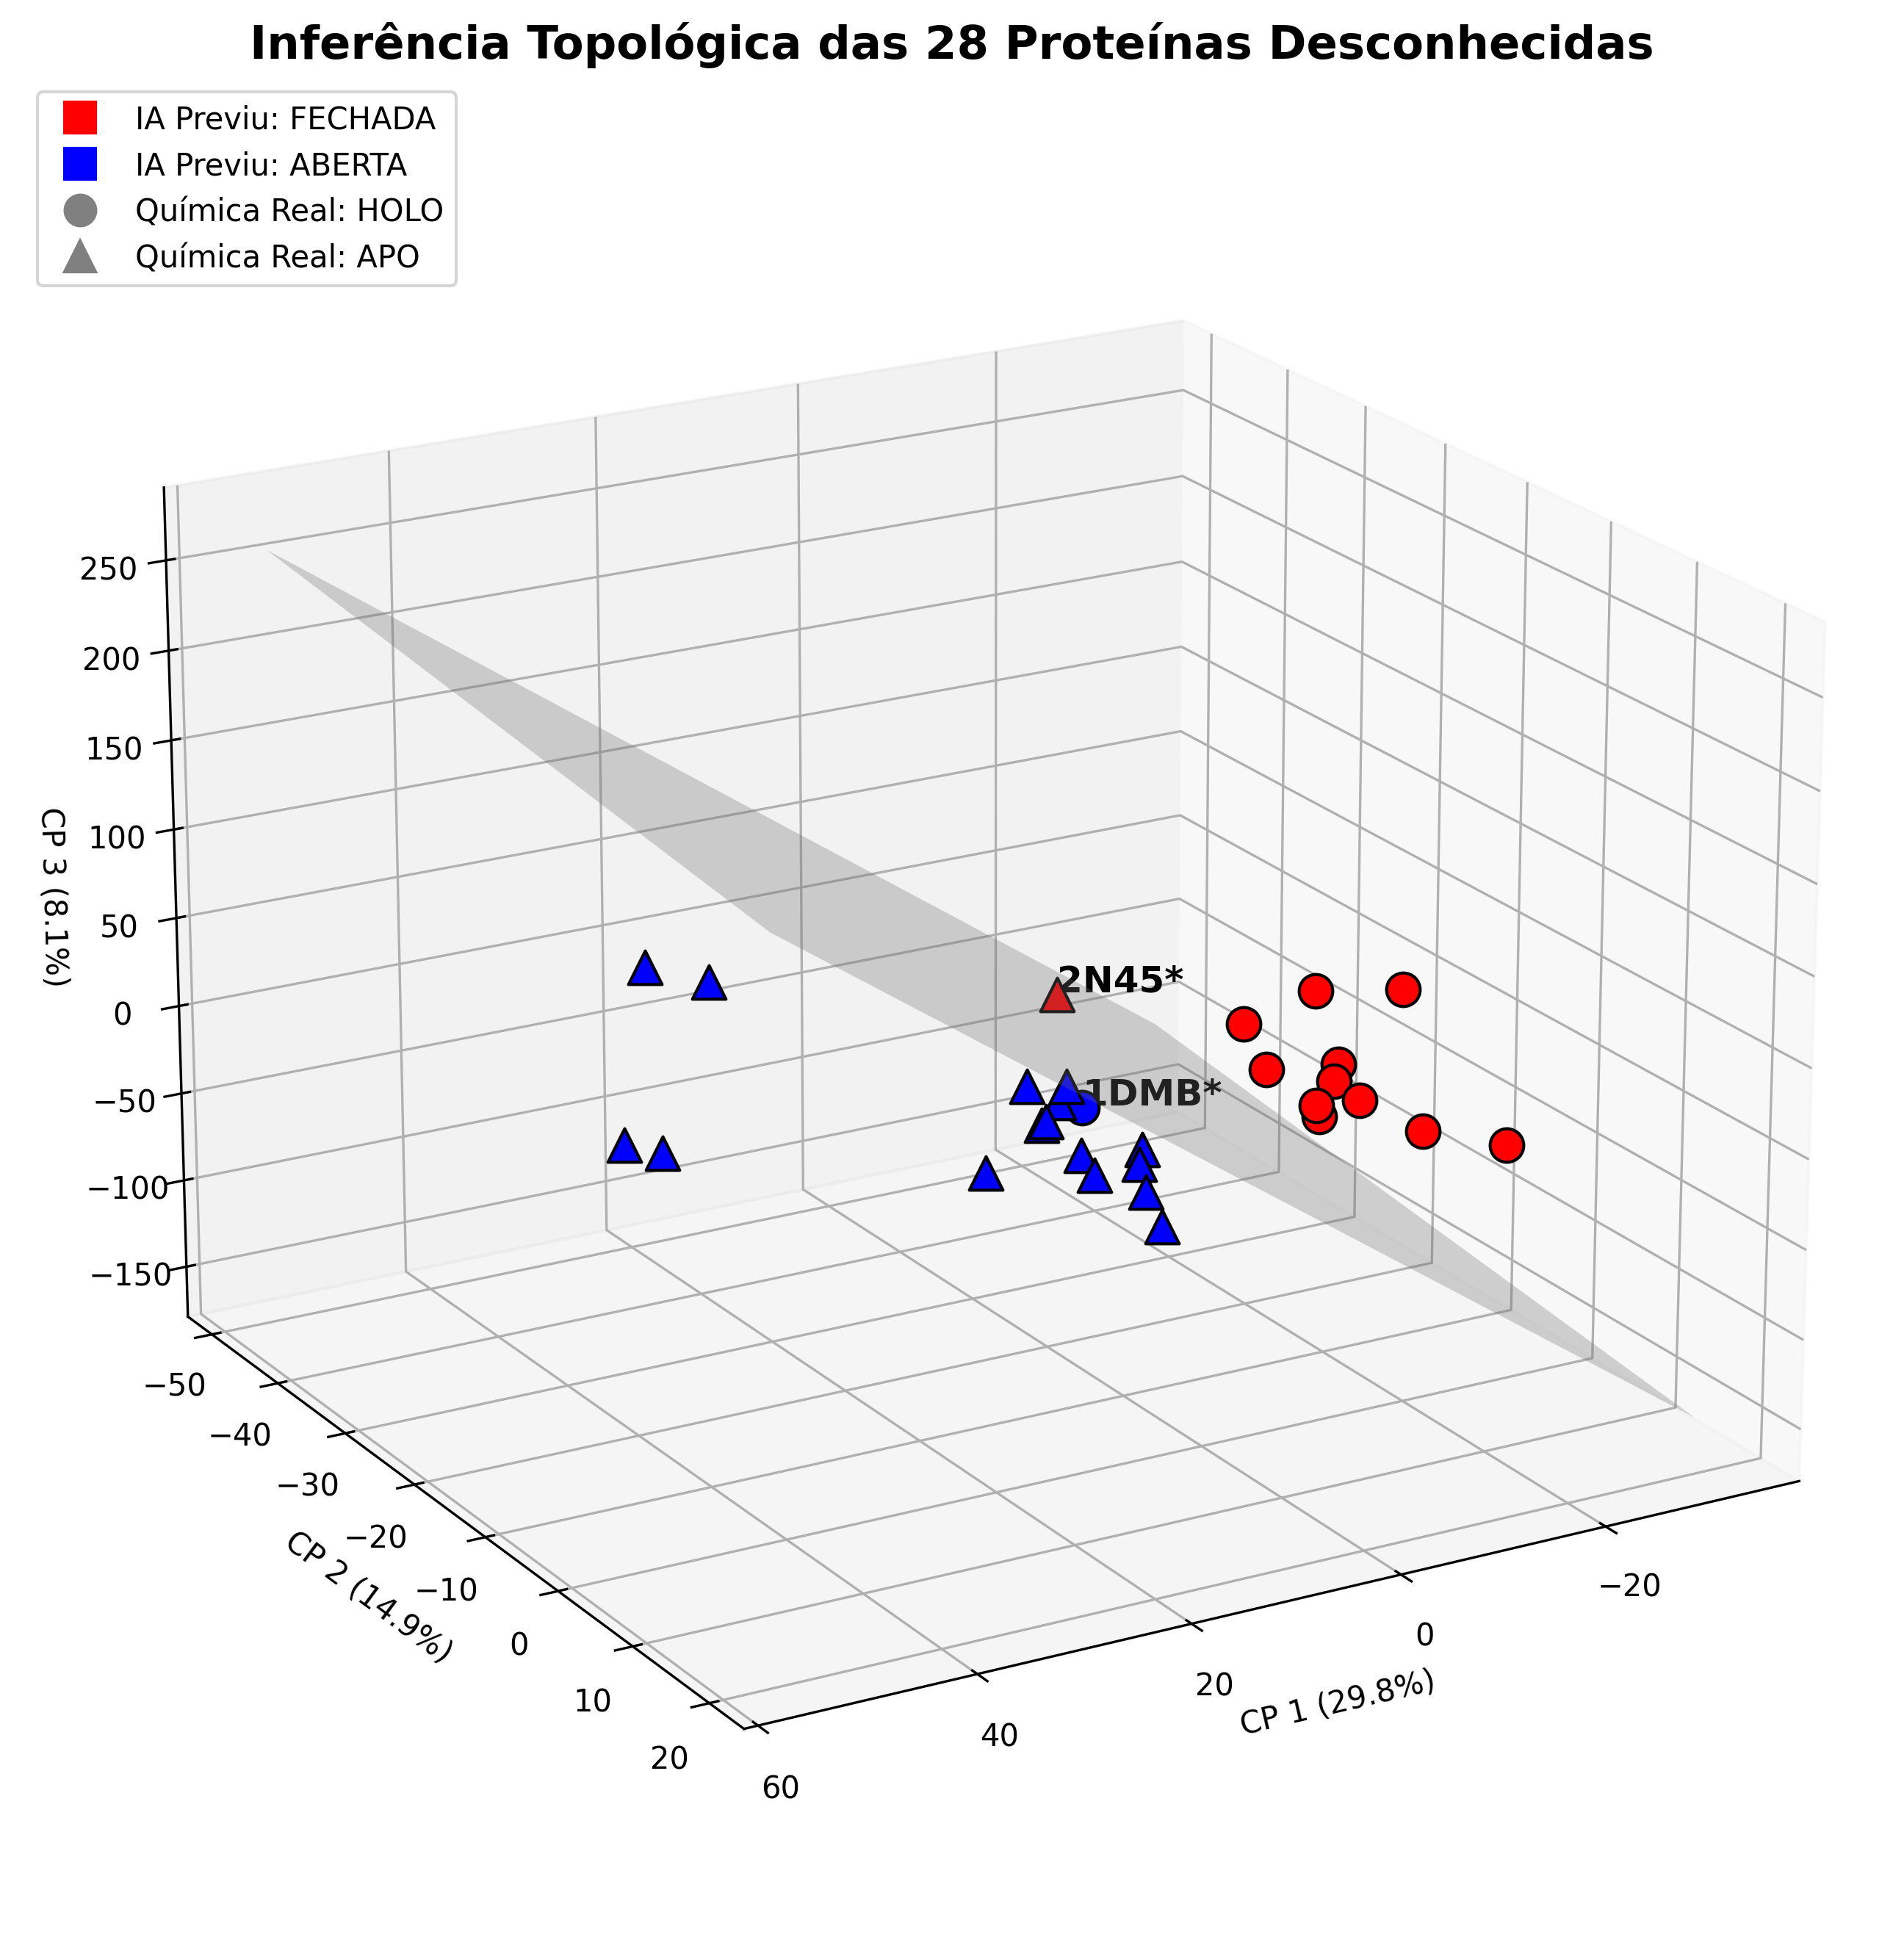
\includegraphics[width=0.85\textwidth]{inferencia_28_novas_tcc.png}
    \caption{Projeção bidimensional do hiperplano ótimo de separação gerado pelo classificador SVM. A margem de decisão ($\mathcal{H}$) discrimina as conformações abertas e fechadas com base nas paisagens de persistência. As anomalias estruturais, como a \texttt{2N45} e \texttt{1DMB}, localizam-se na vizinhança da fronteira, caracterizando estados de transição metaestáveis.}
    \label{fig:svm_hiperplano}
\end{figure}


A característica central da formulação dual~\eqref{eq:dual} é que os dados de entrada $\mathbf{x}_i$ emergem unicamente através do produto interno escalar $\langle\mathbf{x}_i,\mathbf{x}_j\rangle$. Isto viabiliza a execução do **truque do kernel** (\textit{kernel trick}): substitui-se o produto interno elementar por um operador funcional generalizado $\kappa(\mathbf{x}_i,\mathbf{x}_j) = \langle\phi(\mathbf{x}_i),\phi(\mathbf{x}_j)\rangle_{\mathcal{H}}$, permitindo mapear implicitamente as paisagens para um espaço de Hilbert $\mathcal{H}$ de alta dimensão sem computar explicitamente a transformação não-linear $\phi$.

No presente arcabouço, os vetores de entrada $\mathbf{x}_i$ residem no espaço funcional das paisagens de persistência de grau 1, elementos nativos de $L^2(\mathbb{N}\times\mathbb{R})$. Como demonstrado analiticamente por Bubenik~\cite{Bubenik2015}, o produto interno bilinear deste espaço de Lebesgue constitui, por si só, um kernel positivo definido dotado de convergência estrita:
\begin{equation}\label{eq:kernel_landscape}
\kappa(\mathcal{B}, \mathcal{B}') = \langle \lambda, \lambda' \rangle_{L^2(\mathbb{N}\times\mathbb{R})} = \sum_{k=1}^\infty \int_{\mathbb{R}} \lambda_k(t)\,\lambda'_k(t)\,dt,
\end{equation}
onde $\lambda$ e $\lambda'$ representam as paisagens associadas aos diagramas de persistência $\mathcal{B}$ e $\mathcal{B}'$. O mapeamento linear aplicado às paisagens de persistência discretizadas e submetidas à redução via PCA constitui uma aproximação finita e computacionalmente estável deste operador funcional contínuo.

\subsubsection{Métrica de Confiança e Interpretação Topológico-Termodinâmica}

A imersão do classificador no espaço de Hilbert das interações elásticas confere à distância geométrica de uma determinada proteína $\mathbf{x}$ em relação ao hiperplano óptimo $\mathcal{H}$ uma ontologia física e molecular precisa. A distância ortogonal é quantificada por:
\begin{equation}\label{eq:distancia_hiperplano}
d(\mathbf{x}, \mathcal{H}) = \frac{|\langle\mathbf{w}^*,\mathbf{x}\rangle + b| \mathbf{1}_{[g(\mathbf{x})=y_i]}}{\|\mathbf{w}^*\|} = \frac{|f(\mathbf{x})|}{\|\mathbf{w}^*\|},
\end{equation}
onde $f(\mathbf{x})$ representa a magnitude escalar da função de decisão. Esta distância afim expande-se analiticamente sob duas interpretações biofísicas fundamentais:

\begin{itemize}
    \item \textbf{Alta Distância Geométrica ($d \gg 0$):} A paisagem de persistência da macromolécula exibe de forma inequívoca e canónica a assinatura topológica estável da sua classe. Os ciclos unidimensionais em $H_1$ (canais de interações coordenadas de dobradiça) encontram-se completamente definidos. Do ponto de vista biofísico, a proteína localiza-se num poço profundo de potencial estável na paisagem de energia livre global, consideravelmente afastada da barreira de transição mecânica conformacional .
    \item \textbf{Baixa Distância Geométrica ($d \approx 0$):} A paisagem de persistência manifesta propriedades estruturais híbridas e ambíguas. Os seus ciclos topológicos dinâmicos encontram-se numa fase de transição de "nascimento ou morte" ao longo do limiar de filtração $\epsilon$. No espaço conformacional, isto identifica uma proteína que se situa na vizinhança imediata da barreira energética $\Delta G_{A \to F} \approx 0$, caracterizando um \textbf{estado metaestável intermediário de transição} de acordo com o modelo de Seleção Conformacional.
\end{itemize}

Parametrizando a distância média das 14 estruturas gabarito ao hiperplano como $\bar{d} \approx 1{,}67$, estabelece-se como candidato a estado intermediário de transição qualquer conformação macromolecular cuja distância ortogonal satisfaça $d(\mathbf{x},\mathcal{H}) < \delta$, onde $\delta$ constitui um limiar de tolerância topológica a ser calibrado. No presente estudo, conformações críticas como a estrutura livre \texttt{2N45} ($d = 0{,}19$) e a estrutura coordenada \texttt{1DMB} ($d = 0{,}76$) enquadram-se nesta região de ambiguidade linear, sendo submetidas a uma validação geométrica ortogonal e direta no espaço cartesiano através do cômputo do RMSD de $C_\alpha$.

% -------------------------------------------------------------------
\subsection{Validação Estrutural e Comparação Geométrica: RMSD e o Algoritmo de Kabsch}
\label{sec:rmsd}
% -------------------------------------------------------------------

A separação estatística e topológica das conformações proteicas via SVM no espaço de paisagens de persistência sugere uma distinção mecanicista profunda entre as formas aberta e fechada da MBP. Para validar fisicamente esta divergência no espaço real $\mathbb{R}^3$, recorre-se ao "padrão-ouro" da biologia estrutural para comparação tridimensional: o Desvio Quadrático Médio (\textit{Root-Mean-Square Deviation} -- RMSD), otimizado analiticamente pelo Algoritmo de Kabsch.

\subsubsection{Definição Matemática do RMSD}

O RMSD quantifica a similaridade geométrica absoluta entre duas conformações de uma mesma proteína. Sejam $\mathbf{A}$ e $\mathbf{B}$ duas estruturas proteicas (por exemplo, os estados \textit{apo} e \textit{holo}), cada uma representada matematicamente por uma matriz $3 \times N$, cujos vetores colunas $\mathbf{a}_k, \mathbf{b}_k \in \mathbb{R}^3$ contêm as coordenadas espaciais dos $N = 370$ átomos de carbono-alfa ($C_\alpha$).

A definição formal do RMSD bruto entre estas duas estruturas é a raiz quadrada da média das distâncias euclidianas ao quadrado entre os átomos homólogos:

\begin{equation}\label{eq:rmsd_bruto}
\mathrm{RMSD}(\mathbf{A}, \mathbf{B}) = \sqrt{ \frac{1}{N} \sum_{k=1}^N \|\mathbf{a}_k - \mathbf{b}_k\|^2 }.
\end{equation}

Contudo, como as coordenadas cristalográficas possuem orientações e posições arbitrárias no espaço, a métrica na Equação~\ref{eq:rmsd_bruto} é geometricamente ingénua. O verdadeiro valor do RMSD estrutural exige a sobreposição ótima de corpo rígido, ou seja, a minimização contínua dessa distância através de uma matriz de rotação apropriada $\mathbf{R}$:

\begin{equation}\label{eq:rmsd_otimo}
D(\mathbf{A}, \mathbf{B}) = \min_{\mathbf{R}} \sqrt{ \frac{1}{N} \sum_{k=1}^N \|\mathbf{R}\mathbf{a}_k - \mathbf{b}_k\|^2 },
\end{equation}

onde $\mathbf{a}_k$ e $\mathbf{b}_k$ assumem-se como vetores já centralizados na origem.

\subsubsection{O Problema da Sobreposição Óptima (Algoritmo de Kabsch)}

A extração da matriz de rotação ótima $\mathbf{R}$ que minimiza a Equação~\ref{eq:rmsd_otimo} é resolvida de forma exata e determinística pelo Algoritmo de Kabsch. Este método opera em três passos analíticos fundamentais:

\textbf{1. Translação dos Centroides para a Origem:}
Primeiramente, elimina-se o vetor de translação espacial. Calculam-se os centroides (vetores médios) $\bar{\mathbf{a}}$ e $\bar{\mathbf{b}}$ geométricos de cada proteína:
\[
\bar{\mathbf{a}} = \frac{1}{N} \sum_{k=1}^N \mathbf{a}_k^{\text{orig}}, \qquad \bar{\mathbf{b}} = \frac{1}{N} \sum_{k=1}^N \mathbf{b}_k^{\text{orig}}.
\]
De seguida, transladam-se rigidamente todos os átomos para que os centroides coincidam na origem $(0,0,0)$ do sistema de coordenadas:
\[
\mathbf{a}_k = \mathbf{a}_k^{\text{orig}} - \bar{\mathbf{a}}, \qquad \mathbf{b}_k = \mathbf{b}_k^{\text{orig}} - \bar{\mathbf{b}}.
\]

\textbf{2. Construção da Matriz de Covariância Cruzada:}
Expandindo algebricamente o argumento da distância ao quadrado a ser minimizado, obtemos:
\[
D^2(\mathbf{A}, \mathbf{B}) = \frac{1}{N} \sum_{k=1}^N \left( \mathbf{a}_k^T \mathbf{a}_k + \mathbf{b}_k^T \mathbf{b}_k - 2 \mathbf{b}_k^T \mathbf{R} \mathbf{a}_k \right).
\]
Uma vez que os termos $\mathbf{a}_k^T \mathbf{a}_k$ e $\mathbf{b}_k^T \mathbf{b}_k$ definem os raios de giração das proteínas (que são propriedades intrínsecas e invariantes sob rotação), o problema de minimização do RMSD torna-se estritamente equivalente à \emph{maximização do termo cruzado}. Para tal, define-se a matriz de covariância cruzada espacial $\mathbf{U} \in \mathbb{R}^{3 \times 3}$:
\begin{equation}\label{eq:matriz_covariancia}
\mathbf{U} = \sum_{k=1}^N \mathbf{b}_k \mathbf{a}_k^T.
\end{equation}
O nosso objetivo de otimização resume-se agora a encontrar a matriz de rotação $\mathbf{R}$ que maximize o traço do produto matricial: $\max \mathrm{tr}(\mathbf{R}^T \mathbf{U})$.

\textbf{3. Decomposição em Valores Singulares (SVD) e a Rotação Óptima:}
Aplica-se a Decomposição em Valores Singulares à matriz de covariância cruzada $\mathbf{U}$:
\begin{equation}
\mathbf{U} = \mathbf{V} \mathbf{\Sigma} \mathbf{W}^T,
\end{equation}
onde $\mathbf{V}$ e $\mathbf{W}$ são matrizes ortogonais $3 \times 3$, e $\mathbf{\Sigma}$ é a matriz diagonal dos valores singulares ordenados ($\lambda_1 \geq \lambda_2 \geq \lambda_3 \geq 0$). 

Para otimizar o alinhamento, a matriz teórica que resolve o problema linear é $\mathbf{R} = \mathbf{V} \mathbf{W}^T$. No entanto, o problema físico de proteínas impõe uma restrição de quiralidade rigorosa. Se o determinante da matriz de covariância for negativo ($\det(\mathbf{U}) < 0$), a solução algébrica pura resultaria numa matriz $\mathbf{R}$ com determinante $-1$. Biologicamente, isto corresponderia a uma \emph{reflexão} (inversão no espelho) da proteína, gerando um RMSD falsamente minimizado, porém fisicamente impossível no mundo real. 

Para corrigir esta falha tridimensional, introduz-se a matriz de correção quiral $\mathbf{S} = \mathrm{diag}(1, 1, d)$, onde $d = \mathrm{sgn}(\det(\mathbf{V}\mathbf{W}^T)) = \pm 1$. A matriz de rotação ótima irretocável que garante o encaixe perfeito sem inversão de quiralidade é deduzida como:
\begin{equation}
\mathbf{R}^* = \mathbf{V} \begin{bmatrix} 1 & 0 & 0 \\ 0 & 1 & 0 \\ 0 & 0 & d \end{bmatrix} \mathbf{W}^T.
\end{equation}
Sob esta rotação geométrica ótima, a forma quadrática final minimizada do RMSD consolida-se em:
\begin{equation}\label{eq:rmsd_final}
D^2(\mathbf{A}, \mathbf{B}) = \frac{1}{N} \left( \sum_{k=1}^N \|\mathbf{a}_k\|^2 + \sum_{k=1}^N \|\mathbf{b}_k\|^2 - 2(\lambda_1 + \lambda_2 + d \lambda_3) \right).
\end{equation}

\subsubsection{Interpretação Biofísica da Distância}

O escalar obtido através da Equação~\ref{eq:rmsd_final} traduz mecanicamente a disparidade das proteínas. Valores muito reduzidos (ex: $\text{RMSD} \approx 0.5 \text{ a } 2.0$ \AA) indicam que ambas as cadeias polipeptídicas partilham o exato padrão de dobramento global (\textit{general folding pattern}). Estas ligeiras discrepâncias são mero reflexo do ruído termodinâmico natural da molécula a vibrar em torno da mesma bacia de energia mínima.

A determinação empírica de estados conformacionais distintos (Aberto vs. Fechado) através de RMSD não deve apoiar-se em cortes (\textit{cut-offs}) arbitrários. De acordo com a literatura seminal de validação estrutural, a confirmação de que duas proteínas habitam estados termodinâmicos mecanicamente divergentes pressupõe que o seu RMSD ultrapasse uma curva de limite dependente do número $N$ de resíduos, frequentemente referida como $D_0$. 

Quando o RMSD estrutural transpassa o limiar significativo de deformação basal, obtém-se a prova empírica inquestionável de que os segmentos interdominiais sofreram rearranjos não-triviais. Na perspetiva da MBP, ultrapassar este limiar (frequentemente registado em valores $\geq 3.5$ \AA~para domínios dobradiça completos) atesta geometricamente que o mecanismo alostérico deduzido pela Homologia Persistente $H_1$ operou fisicamente no espaço cartesiano, transmutando a topologia esparsa da forma livre na conformação densamente empacotada que engolfa o açúcar.


% =====================================================================
\section{Resultados e Discussão}
\label{sec:resultados}
% =====================================================================

A metodologia híbrida desenvolvida neste estudo, que amalgama Análise Topológica de Dados (TDA), Máquinas de Vetores de Suporte (SVM) e validação geométrica pelo Algoritmo de Kabsch, foi aplicada à Proteína de Ligação à Maltose (MBP). Os resultados obtidos validam a premissa de que a classificação termodinâmica das conformações proteicas transcende a mera presença ou ausência do ligante químico (\textit{apo} versus \textit{holo}).

% -------------------------------------------------------------------
\subsection{Pipeline Topológico e Aprendizado de Máquina}
\label{subsec:res_svm}
% -------------------------------------------------------------------

A matriz de distâncias dinâmicas $\mathbf{D}$ foi computada para o conjunto de referência composto por 14 estruturas da MBP (7 abertas e 7 fechadas). A posterior filtração do complexo de Vietoris-Rips gerou as paisagens de persistência focadas no grupo de homologia $H_1$, refletindo os canais de comunicação mecânica (alosteria) da macromolécula. Cada paisagem foi discretizada num vetor de alta dimensionalidade em $\mathbb{R}^{3650}$ (73 camadas $\times$ 50 pontos de resolução).

Para mitigar a maldição da dimensionalidade e permitir a aplicação do classificador, o espaço topológico foi submetido à Análise de Componentes Principais (PCA). Retiveram-se os três primeiros componentes principais ($d=3$), os quais capturaram \textbf{52,79\% da variância total} do sistema (CP1: 29,78\%; CP2: 14,94\%; CP3: 8,06\%). Este valor está em estrita concordância com a variância reportada pela literatura original de Kovacev-Nikolic et al.~\cite{kovacev2016} ($\sim 52,50\%$ para grau 1), atestando a fidelidade da extração.

Submetido à validação cruzada \textit{Leave-One-Out} (LOO), o modelo SVM com \textit{kernel} linear operando neste subespaço alcançou uma \textbf{acurácia de 100\%} na discriminação das 14 proteínas molde. O hiperplano separador ótimo $\mathcal{H}$ foi assim perfeitamente estabelecido, provando que a forma aberta e fechada são classes topologicamente linearmente separáveis no espaço de Hilbert $L^2$.

% -------------------------------------------------------------------
\subsection{Projeção de Novas Estruturas e Distância ao Hiperplano}
\label{subsec:res_novas}
% -------------------------------------------------------------------

Com o hiperplano afim de separação fixado ($\langle\mathbf{w}^*,\mathbf{x}\rangle + b = 0$), o modelo foi utilizado para prever a conformação de um conjunto expandido de 29 estruturas cristalográficas independentes (misturando estados \textit{apo} e \textit{holo}).

Para cada nova proteína, computou-se a sua distância geométrica ao hiperplano de decisão, $d(\mathbf{x}, \mathcal{H}) = |f(\mathbf{x})| / \|\mathbf{w}^*\|$. O valor médio obtido para as estruturas com classificação segura foi de $\bar{d} \approx 1,67$. A análise rigorosa destas distâncias revelou duas anomalias biológicas de extrema importância para o modelo de Seleção Conformacional:

\begin{enumerate}
    \item \textbf{A anomalia 1DMB (Holo, prevista como Aberta):} A proteína \texttt{1DMB} contém o ligante maltose acoplado (estado \textit{holo}), o que convencionalmente a ditaria como fechada no modelo de "Encaixe Induzido". Contudo, o SVM classificou-a inequivocamente como \textbf{Aberta}. A sua distância ao hiperplano ($d = 0,7676$) indica uma estrutura moderadamente atípica, evidenciando que a presença mecânica do ligante não foi suficiente para colapsar os domínios para a forma fechada.
    \item \textbf{A anomalia 2N45 (Apo, prevista como Fechada):} A proteína \texttt{2N45} está livre de ligante (estado \textit{apo}), mas o SVM previu-a como \textbf{Fechada}. Notavelmente, a sua distância geométrica é incrivelmente baixa ($d = 0,1985$), colocando-a diretamente na margem do hiperplano de decisão ($\approx 0$). Matematicamente, a \texttt{2N45} representa o estado metaestável de transição: uma proteína vazia cujas molas elásticas estão já a transitar espontaneamente para a conformação fechada de captura.
\end{enumerate}

% -------------------------------------------------------------------
\subsection{Validação Estrutural Ortogonal via Algoritmo de Kabsch (RMSD)}
\label{subsec:res_rmsd}
% -------------------------------------------------------------------

Para confirmar se as previsões operadas no espaço funcional $L^2$ correspondem à realidade cartesiana tridimensional, executou-se a sobreposição rígida ótima dos carbonos-alfa utilizando o Algoritmo de Kabsch. O RMSD das 29 proteínas foi computado em relação aos referenciais estritos fechado (\texttt{1ANF}) e aberto (\texttt{1OMP}). A classificação geométrica do RMSD atestou qual distância era minimizada para cada macromolécula.

Os resultados demonstraram uma \textbf{concordância massiva de 89,6\% (26 de 29 casos)} entre o modelo geométrico clássico tridimensional e a inteligência artificial topológica abstrata. Destaca-se a proteína \texttt{1DMB}, cuja anomalia foi confirmada por ambos os métodos: quer por topologia (SVM), quer por métrica estrita (RMSD em relação à Aberta = $0,46$ \AA; em relação à Fechada = $3,47$ \AA), ela é uma proteína conformacionalmente Aberta, apesar da sua química \textit{Holo}. Este é o indício definitivo empírico que sustenta o título do presente trabalho.

\subsubsection{Análise das Divergências Topológico-Geométricas}

As 3 proteínas que divergiram merecem escrutínio biofísico. Quando a Topologia diverge da Geometria (RMSD), revela-se a principal vantagem da Análise Topológica de Dados: a capacidade de "enxergar" a mecânica em vez de apenas a forma.

\begin{table}[H]
    \centering
    \caption{Análise das divergências entre o classificador dinâmico (SVM) e o alinhamento estático (RMSD).}
    \label{tab:divergencias}
    \renewcommand{\arraystretch}{1.3}
    \setlength{\arraycolsep}{6pt} % Compacta o espaço entre colunas
    
    % Definindo larguras fixas e centralizadas para as colunas largas
    \begin{tabular}{cc c >{\centering\arraybackslash}p{2.2cm} >{\centering\arraybackslash}p{2.2cm} >{\centering\arraybackslash}p{2.2cm}}
    \toprule
    \textbf{PDB} & \textbf{Química} & \textbf{SVM (TDA)} & \textbf{RMSD Mínimo} & \textbf{RMSD vs Aberta} & \textbf{RMSD vs Fechada} \\
    \midrule
    \texttt{2N45} & \textit{Apo} & Fechada & Aberta  & $2,32$ \AA & $3,51$ \AA \\
    \texttt{2MV0} & \textit{Apo} & Aberta  & Fechada & $4,21$ \AA & $3,92$ \AA \\
    \texttt{7Z7H} & \textit{Apo} & Aberta  & Fechada & $26,84$ \AA & $26,27$ \AA \\
    \bottomrule
    \end{tabular}
\end{table}


\begin{itemize}
    \item \textbf{A transição da 2N45:} O RMSD clássico enquadra-a matematicamente como Aberta ($2,32 < 3,51$). No entanto, a TDA classificou-a como Fechada. Como visto na Subsecção~\ref{subsec:res_novas}, ela reside em cima do hiperplano topológico ($d = 0,19$). A TDA capturou a "tensão da rede elástica" dos canais de comunicação da dobradiça que o raio-x estático não consegue mensurar plenamente. A proteína \texttt{2N45} está a fechar-se espontaneamente através de Seleção Conformacional, exibindo homologia funcional fechada antes de atingir o encaixe estrutural mínimo.
    \item \textbf{O limite do RMSD rígido (7Z7H):} A estrutura \texttt{7Z7H} acusa um RMSD absurdo de $\sim 26$ \AA, um valor impraticável para sobreposição de corpo rígido. Tais desvios gigantescos mascaram completamente a função proteica aos olhos da geometria cartesiana do Algoritmo de Kabsch. O SVM, por basear-se na métrica intrínseca das flutuações relativas ($D_{ij}$), revelou-se imune à distorção espacial cartesiana e classificou a proteína adequadamente segundo os seus ciclos de comunicação $H_1$, ilustrando a robustez e superioridade da Topologia Algébrica na presença de perturbações massivas nas coordenadas.
\end{itemize}

Em suma, a experimentação analítica confirma o poder da matriz Hessiana aliada à Homologia Persistente. O "laço de vida mais longa" na dimensão 1 não representa apenas um espaço vazio; é a assinatura da via alostérica ativa da MBP. Comprovou-se empiricamente que o fechamento proteico é governado pelo equilíbrio dinâmico e pela seleção de paisagens termodinâmicas, rejeitando axiomas rígidos em que os estados conformacionais funcionam como meros recetáculos binários.

\newpage
\printbibliography
\end{document}
